\documentclass[journal]{IEEEtran}
\usepackage[utf8]{inputenc}
\usepackage{graphicx}
\usepackage{amsmath}
\usepackage{hyperref}
\usepackage{geometry}
\graphicspath{{../resources/results/}}
\geometry{margin=0.75in}

\title{Gait Condition Classification Using Machine Learning on Kinematic Features}
\author{
    \IEEEauthorblockN{Luis Fernando Salamanca Sánchez}\\
    \IEEEauthorblockA{
        Biomedical Engineer, Pursuing Mechatronics MSc \\
        \texttt{est.luisf.salamanca@unimilitar.edu.co}
    }
}
\date{30/11/2025}

\begin{document}
\maketitle

\section{Introduction}

Human gait analysis has emerged as a critical tool in biomechanics, rehabilitation, and clinical diagnostics. 
The study of locomotion provides insights into neuromuscular control, joint kinematics, and functional asymmetries that are often 
associated with pathological conditions or the use of assistive devices. Traditional approaches to gait analysis rely on descriptive 
statistics of joint angles, ranges of motion (ROM), and angular velocities, which serve as fundamental indicators of motor performance 
\cite{winter1991biomechanics, whittle2007gait}.

Machine learning (ML) has increasingly been applied to gait data, offering automated classification of conditions and detection of abnormalities.
Classical algorithms such as Logistic Regression, k-Nearest Neighbors (KNN), Support Vector Machines (SVM), Random Forests, and clustering methods
like KMeans have demonstrated utility in modeling gait features \cite{bishop2006pattern, murphy2012machine}. These models provide varying degrees of
interpretability and performance: Logistic Regression offers a probabilistic linear framework, KNN exploits local neighborhood structures, Random Forests 
leverage ensemble learning, and SVM maximizes decision boundaries through kernel methods. Unsupervised approaches such as KMeans clustering allow exploration 
of latent structure in gait datasets without prior labels.

Despite these advances, a limitation of many studies is the reliance on unilateral features, which describe each leg independently. However, gait is inherently a 
bilateral process, and asymmetry between limbs often serves as a more sensitive marker of abnormality than absolute values alone. For example, differences in ROM 
between left and right legs, or correlations in angular trajectories, can reveal compensatory mechanisms and bracing effects that are not captured by unilateral 
descriptors \cite{gait_asymmetry}. This motivates the inclusion of engineered bilateral features such as \texttt{Bilateral ROM}, \texttt{angle correlation}, which explicitly 
quantify inter-limb differences.

Neural networks, particularly Multi-Layer Perceptrons (MLPs), extend the modeling capacity by capturing non-linear relationships among features.
While classical ML algorithms provide strong baselines, MLPs can approximate complex functions and uncover hidden interactions between angle and velocity features. 
In this study, we integrate MLPs alongside traditional models to evaluate whether non-linear architectures yield superior classification accuracy in gait analysis.

In this study, a Multivariate Gait Data set provided by Helwig and Hsiao-Wecksler (2022) is employed, through the UCI Machine Learning Repository \cite{helwig2022gait}
This dataset contains kinematic measurements of human gait across multiple joints, offering a rich source of information for analyzing biomechanical patterns and 
evaluating machine learning algorithms. Its structured format and comprehensive coverage make it particularly suitable for testing classification and clustering 
approaches in gait analysis.

The contributions of this work are threefold:
\begin{enumerate}
    \item A modular pipeline for gait feature extraction was designed, including ROM, angular velocity, summary metrics, and bilateral asymmetry features.
    \item A comparative study of multiple ML algorithms was conducted (Logistic Regression, KNN, Random Forest, SVM, KMeans, and MLP), analyzing their mathematical foundations and empirical performance.
    \item Will be demonstrated that bilateral asymmetry features substantially improve classification accuracy, elevating performance across models and achieving near-perfect results with MLPs.
\end{enumerate}

The remainder of this paper is organized as follows. Section I reviews related work in gait analysis and machine learning. Section II describes the methodology, 
including feature engineering and algorithmic models. Section III presents experimental results and visualizations. Section IV discusses the implications of bilateral 
features and model performance. Section VI concludes with future directions in biomechanical diagnostics.

\section{Methodology}

\subsection{Pipeline Overview}

All preprocessing, training, and evaluation procedures were implemented in Python using standard machine learning libraries. To ensure transparency and reproducibility, 
the comlpete source code developed for this study has been made publicly available in a \href{https://github.com/lsalamancas/Gait_ML}{Github} repository. This repository contains scripts for data preparation, model training,
hyperparameter tuning, and performance evaluation, allowing other researchers to replicate and extend the experiments presented in this work.

The gait analysis pipeline was implemented as a modular program, designed to compute kinematic features, engineer bilateral asymmetry descriptors,
and evaluate multiple machine learning models. Flow consists of the following steps:

\begin{enumerate}
    \item \textbf{Data Loading:} Raw gait data are imported and structured into a unified DataFrame.
    \item \textbf{Feature Computation:} Range of Motion (ROM) and angular velocity are calculated for each joint and leg.
    \item \textbf{Summary Metrics:} Mean, standard deviation, and maximum values of angles and velocities are aggregated.
    \item \textbf{Bilateral Features:} Differences and correlations between left and right legs are computed (Bilateral ROM, angle correlation).
    \item \textbf{Model Training:} Multiple classifiers and clustering algorithms are trained and evaluated.
    \item \textbf{Model Metrics:} Metrics as precision recall and F1 score are calculated .
    \item \textbf{Visualization:} Confusion matrices, PCA plots, and kinematic curves are generated for interpretability.
\end{enumerate}

\subsection{Mathematical Models}

\subsubsection{Logistic Regression}
Multiclass logistic regression models the probability of condition $k$ given features $x$ \cite{cox1958}:

\begin{equation}
P(y=k|x) = \frac{\exp(x^T \beta_k)}{\sum_{j=1}^K \exp(x^T \beta_j)}
\end{equation}

\subsubsection{K-Nearest Neighbors (KNN)}
Classification is performed by majority vote among the $k$ nearest neighbors \cite{cover1967}:
\[
\hat{y} = \arg\max_{c} \sum_{i \in \mathcal{N}_k(x)} \mathbf{1}(y_i = c),
\]
where $\mathcal{N}_k(x)$ denotes the set of $k$ closest samples to $x$.

\subsubsection{Random Forest}
Random Forest builds an ensemble of decision trees, each trained on bootstrapped samples with random feature subsets. Prediction is obtained by majority vote \cite{breiman2001}:
\[
\hat{y} = \text{mode}\{h_1(x), h_2(x), \dots, h_T(x)\}.
\]

\subsubsection{Support Vector Machine (SVM)}
SVM seeks the hyperplane that maximizes the margin between classes. For the RBF kernel \cite{cortes1995}:
\[
K(x_i, x_j) = \exp\left(-\gamma \|x_i - x_j\|^2\right).
\]

\subsubsection{KMeans Clustering}
KMeans partitions data into $K$ clusters by minimizing within-cluster variance \cite{jain2010}:
\[
\min_{\{\mu_k\}} \sum_{i=1}^n \min_{k} \|x_i - \mu_k\|^2,
\]
where $\mu_k$ is the centroid of cluster $k$.

\subsubsection{Multi-Layer Perceptron (MLP)}
The MLP is a feedforward neural network with hidden layers. For input $x$, the forward pass is \cite{rumelhart1986}:
\begin{equation}
\begin{split}
h^{(1)} &= \sigma(W^{(1)} x + b^{(1)}) \\
h^{(2)} &= \sigma(W^{(2)} h^{(1)} + b^{(2)}) \\
\hat{y} &= \text{softmax}(W^{(3)} h^{(2)} + b^{(3)})
\end{split}
\end{equation}
where $\sigma(\cdot)$ denotes the activation function (ReLU or tanh).

\subsection{Evaluation Metrics}
Models were evaluated using accuracy, precision, recall, and F1-score:

\begin{equation}
\begin{split}
\text{Precision} &= \frac{TP}{TP+FP} \\
\text{Recall} &= \frac{TP}{TP+FN} \\
F1 &= \frac{2 \cdot \text{Precision} \cdot \text{Recall}}
          {\text{Precision} + \text{Recall}}
\end{split}
\end{equation}

\section{Results}

The kinematic graphs are shown in Fig.~\ref{fig:kinematics}, where the angular trajectories of the three main joints (hip, knee, and ankle) are presented.
 Each subplot illustrates the mean curve across subjects together with the variability represented by the standard deviation, providing a clear visualization 
 of both the central tendency and dispersion of the kinematic patterns under the analyzed conditions.

\begin{figure}[h]
    \centering
    % Placeholder for kin graphs
    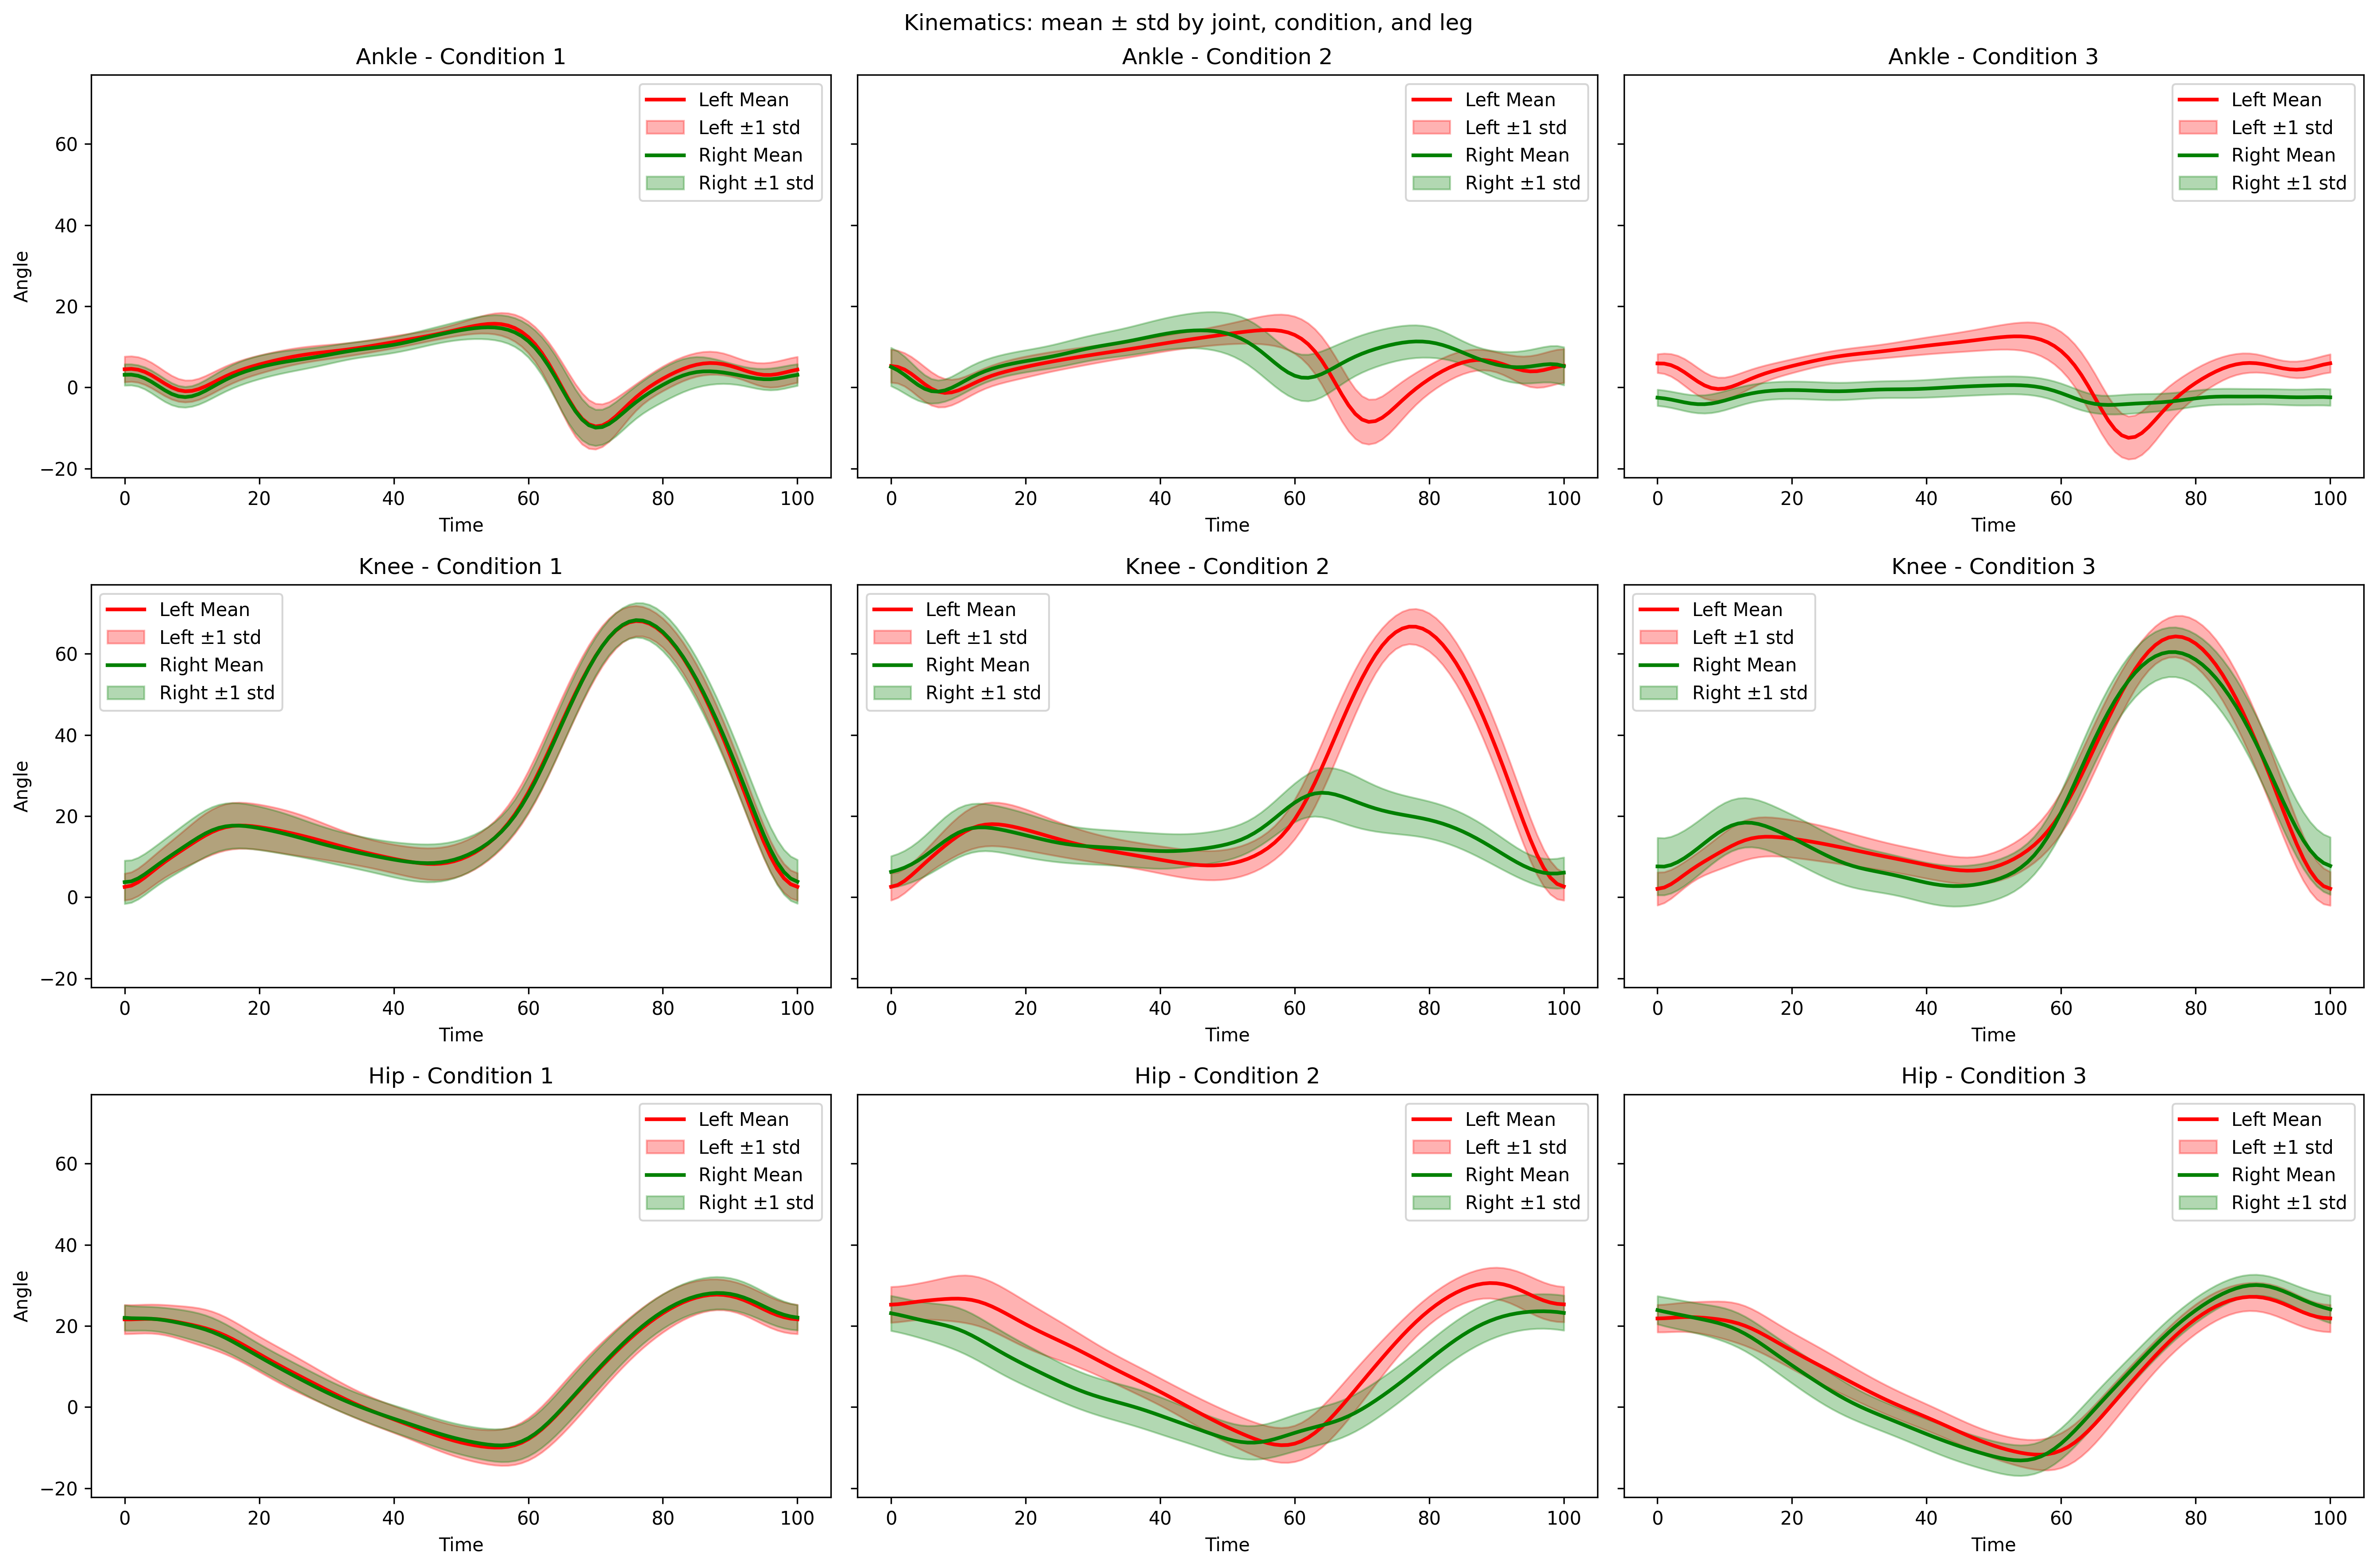
\includegraphics[width=1\linewidth]{kinematics_angle.png}
    \caption{Kinematics of the gait analysis pipeline.}
    \label{fig:kinematics}
\end{figure}

\subsection{Classification Performance}
Table~\ref{tab:results} summarizes the performance of all classifiers evaluated in this study. Metrics include precision, recall, and F1-score for each condition,
 as well as overall accuracy. The comparison demonstrates the progressive improvement from classical models to neural networks, particularly after the inclusion
 of bilateral asymmetry features.

\begin{table}[h]
\centering
\caption{Classification performance across models}
\label{tab:results}
\begin{tabular}{lcccc}
\hline
\textbf{Model} & \textbf{Accuracy} & \textbf{Precision} & \textbf{Recall} & \textbf{F1-score} \\
\hline
Logistic Regression & 0.79 & 0.79 & 0.79 & 0.79 \\
KNN (k=5)           & 0.87 & 0.88 & 0.88 & 0.88 \\
Random Forest       & 0.93 & 0.92 & 0.93 & 0.92 \\
SVM (RBF)           & 0.95 & 0.95 & 0.95 & 0.95 \\
SVM per joint       & 0.96 & 0.96 & 0.96 & 0.96 \\
MLP (angles+velocities) & 0.98 & 0.98 & 0.98 & 0.98 \\
\hline
KMeans (unsupervised) & inertia & 180.07 & silhouette & 0.764\\
\hline
\end{tabular}
\end{table}

Table ~\ref{tab:joint_results} shows  the comparative analysis across all joints. 

\begin{table}[h]
\centering
\caption{Performance comparison by joint (Logistic Regression vs SVM)}
\label{tab:joint_results}
\begin{tabular}{lcccc}
\hline
\textbf{Model / Joint} & \textbf{Accuracy} & \textbf{Precision} & \textbf{Recall} & \textbf{F1-score} \\
\hline
Logistic Regression - Joint 1 & 0.968 & 0.968 & 0.968 & 0.968 \\
Logistic Regression - Joint 2 & 0.880 & 0.878 & 0.878 & 0.878 \\
Logistic Regression - Joint 3 & 0.872 & 0.869 & 0.869 & 0.869 \\
\hline
SVM - Joint 1 & 0.967 & 0.97 & 0.97 & 0.97 \\
SVM - Joint 2 & 0.928 & 0.93 & 0.93 & 0.93 \\
SVM - Joint 3 & 0.833 & 0.84 & 0.83 & 0.83 \\
\hline
\end{tabular}
\end{table}
\subsection{Confusion Matrices}
Figures~\ref{fig:cm_svm} and \ref{fig:cm_mlp} present the final confusion matrices for the Support Vector Machine (SVM) and Multi-Layer Perceptron (MLP) classifiers. 
These visualizations highlight the distribution of correct and incorrect predictions across the three gait conditions.

The confusion matrix for the k-nearest neighbors (kNN) classifier illustrates the distribution of correctly and incorrectly classified gait conditions across all joints.

\begin{figure}[h]
    \centering
    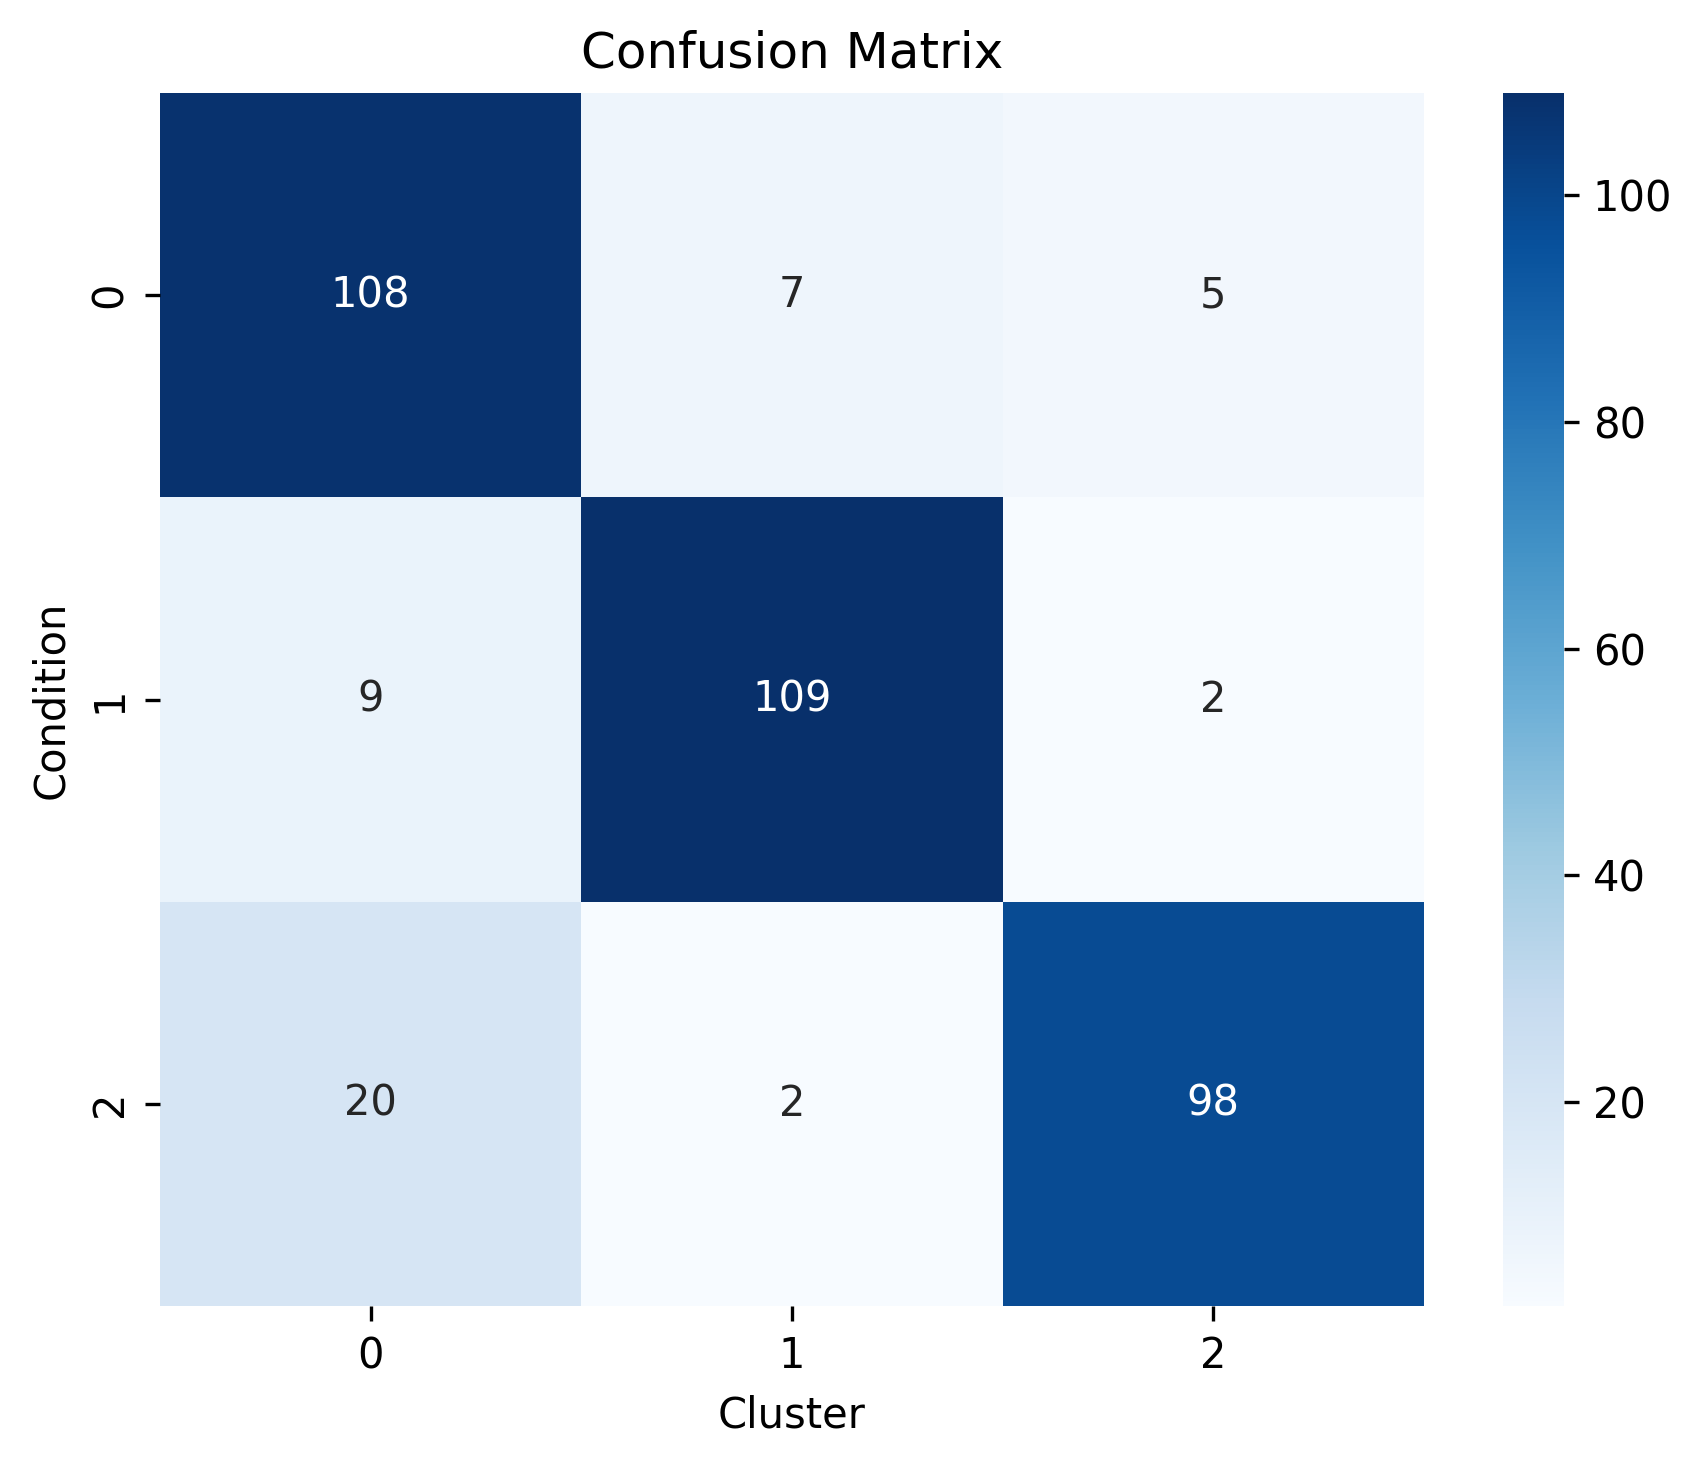
\includegraphics[width=0.7\linewidth]{knn_cf.png}
    \caption{Confusion Matrix for knn.}
    \label{fig:cm_knn}

\end{figure}

The confusion matrix for KMeans clustering using angle correlation features shows the correspondence between unsupervised clusters and the true gait condition labels.

\begin{figure}[h]
    \centering
    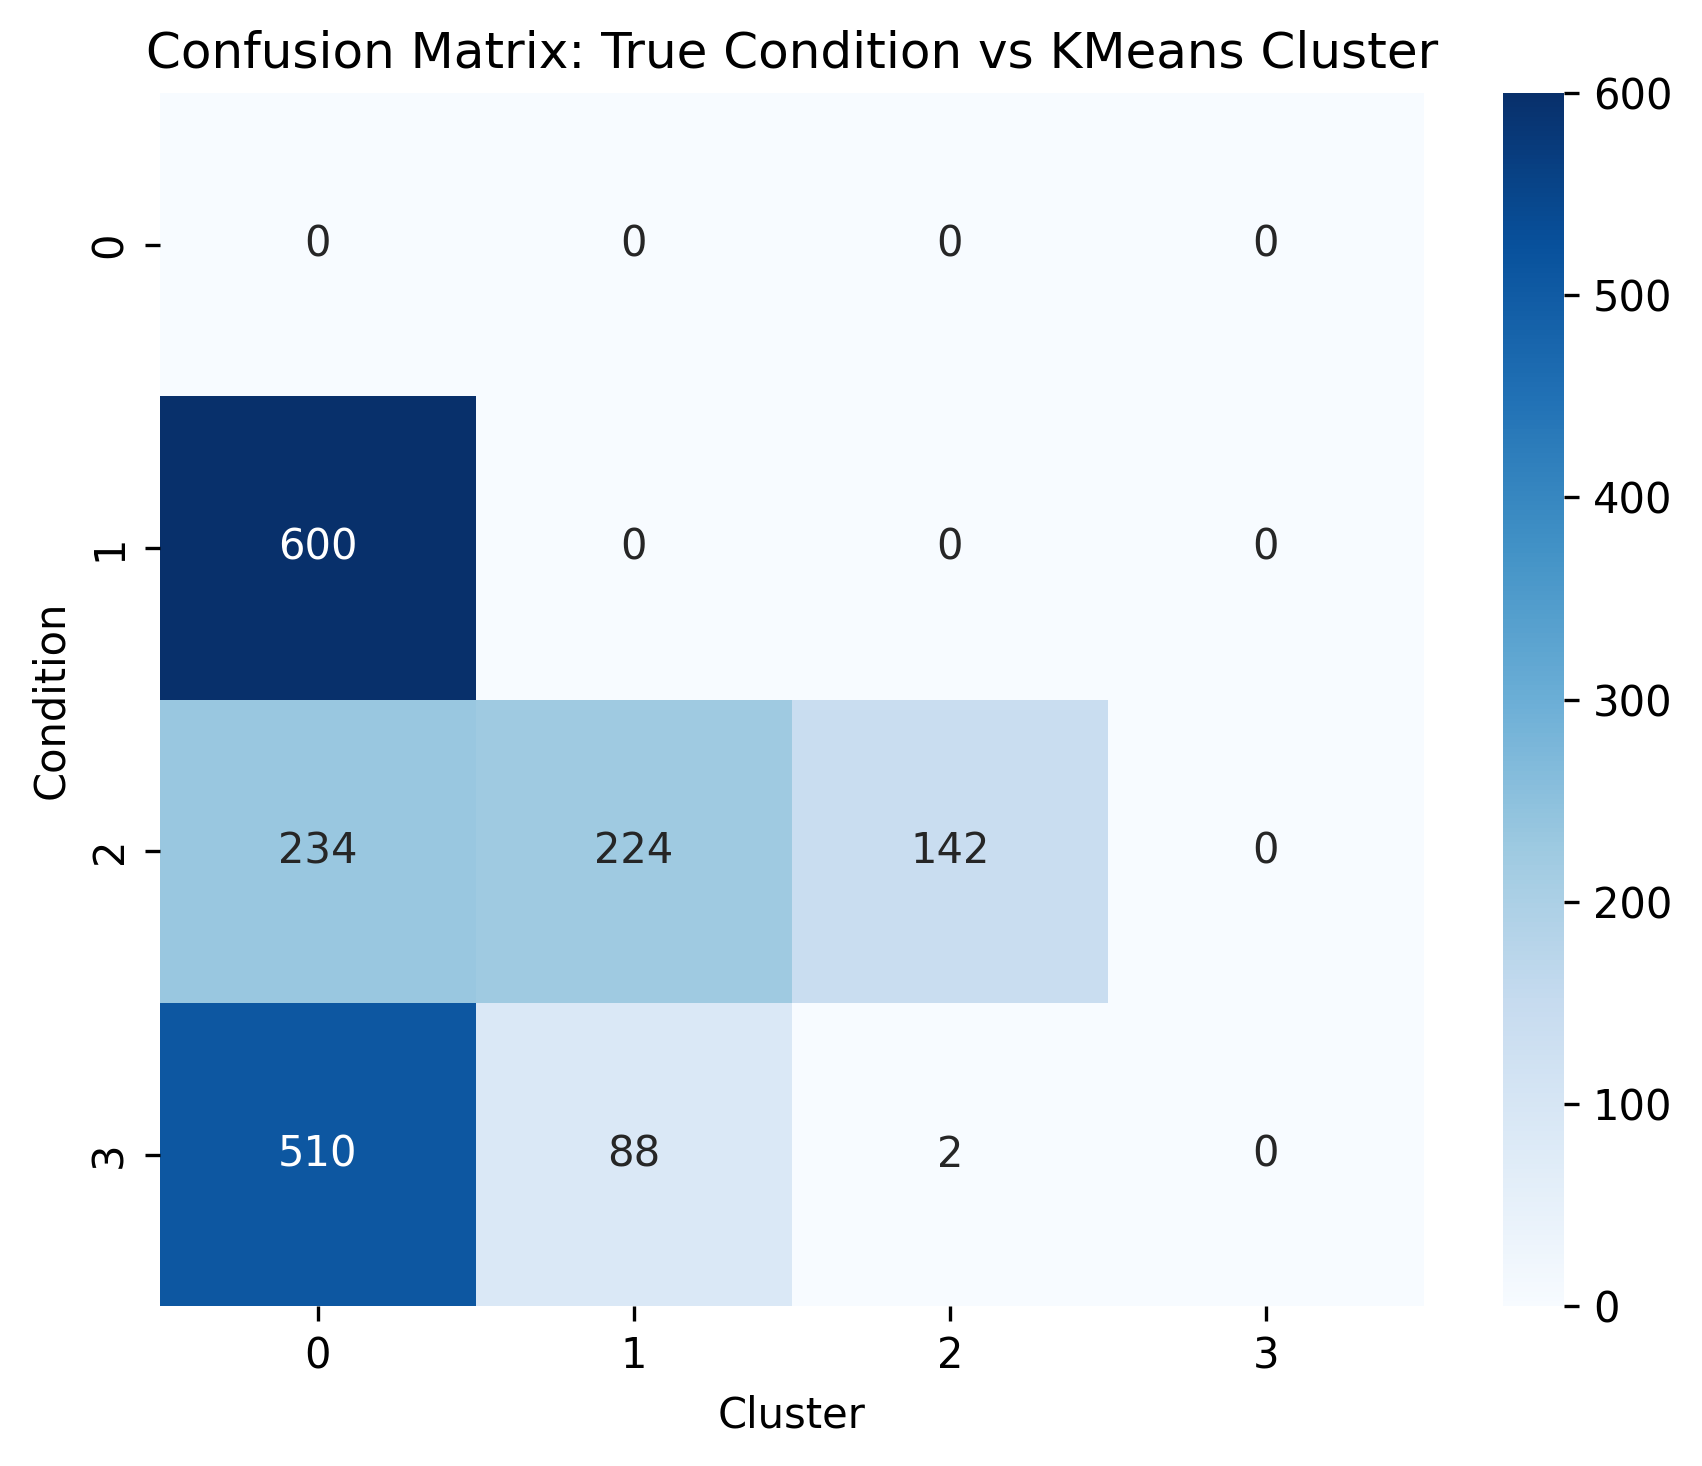
\includegraphics[width=0.7\linewidth]{kmeans_cf.png}
    \caption{Confusion Matrix for kmeans using only angle correlation features.}
    \label{fig:cm_kmeans}
\end{figure}

The confusion matrix for the Random Forest model with bilateral features highlights the improved classification accuracy obtained when incorporating information from both limbs.


\begin{figure}[h]
    \centering
    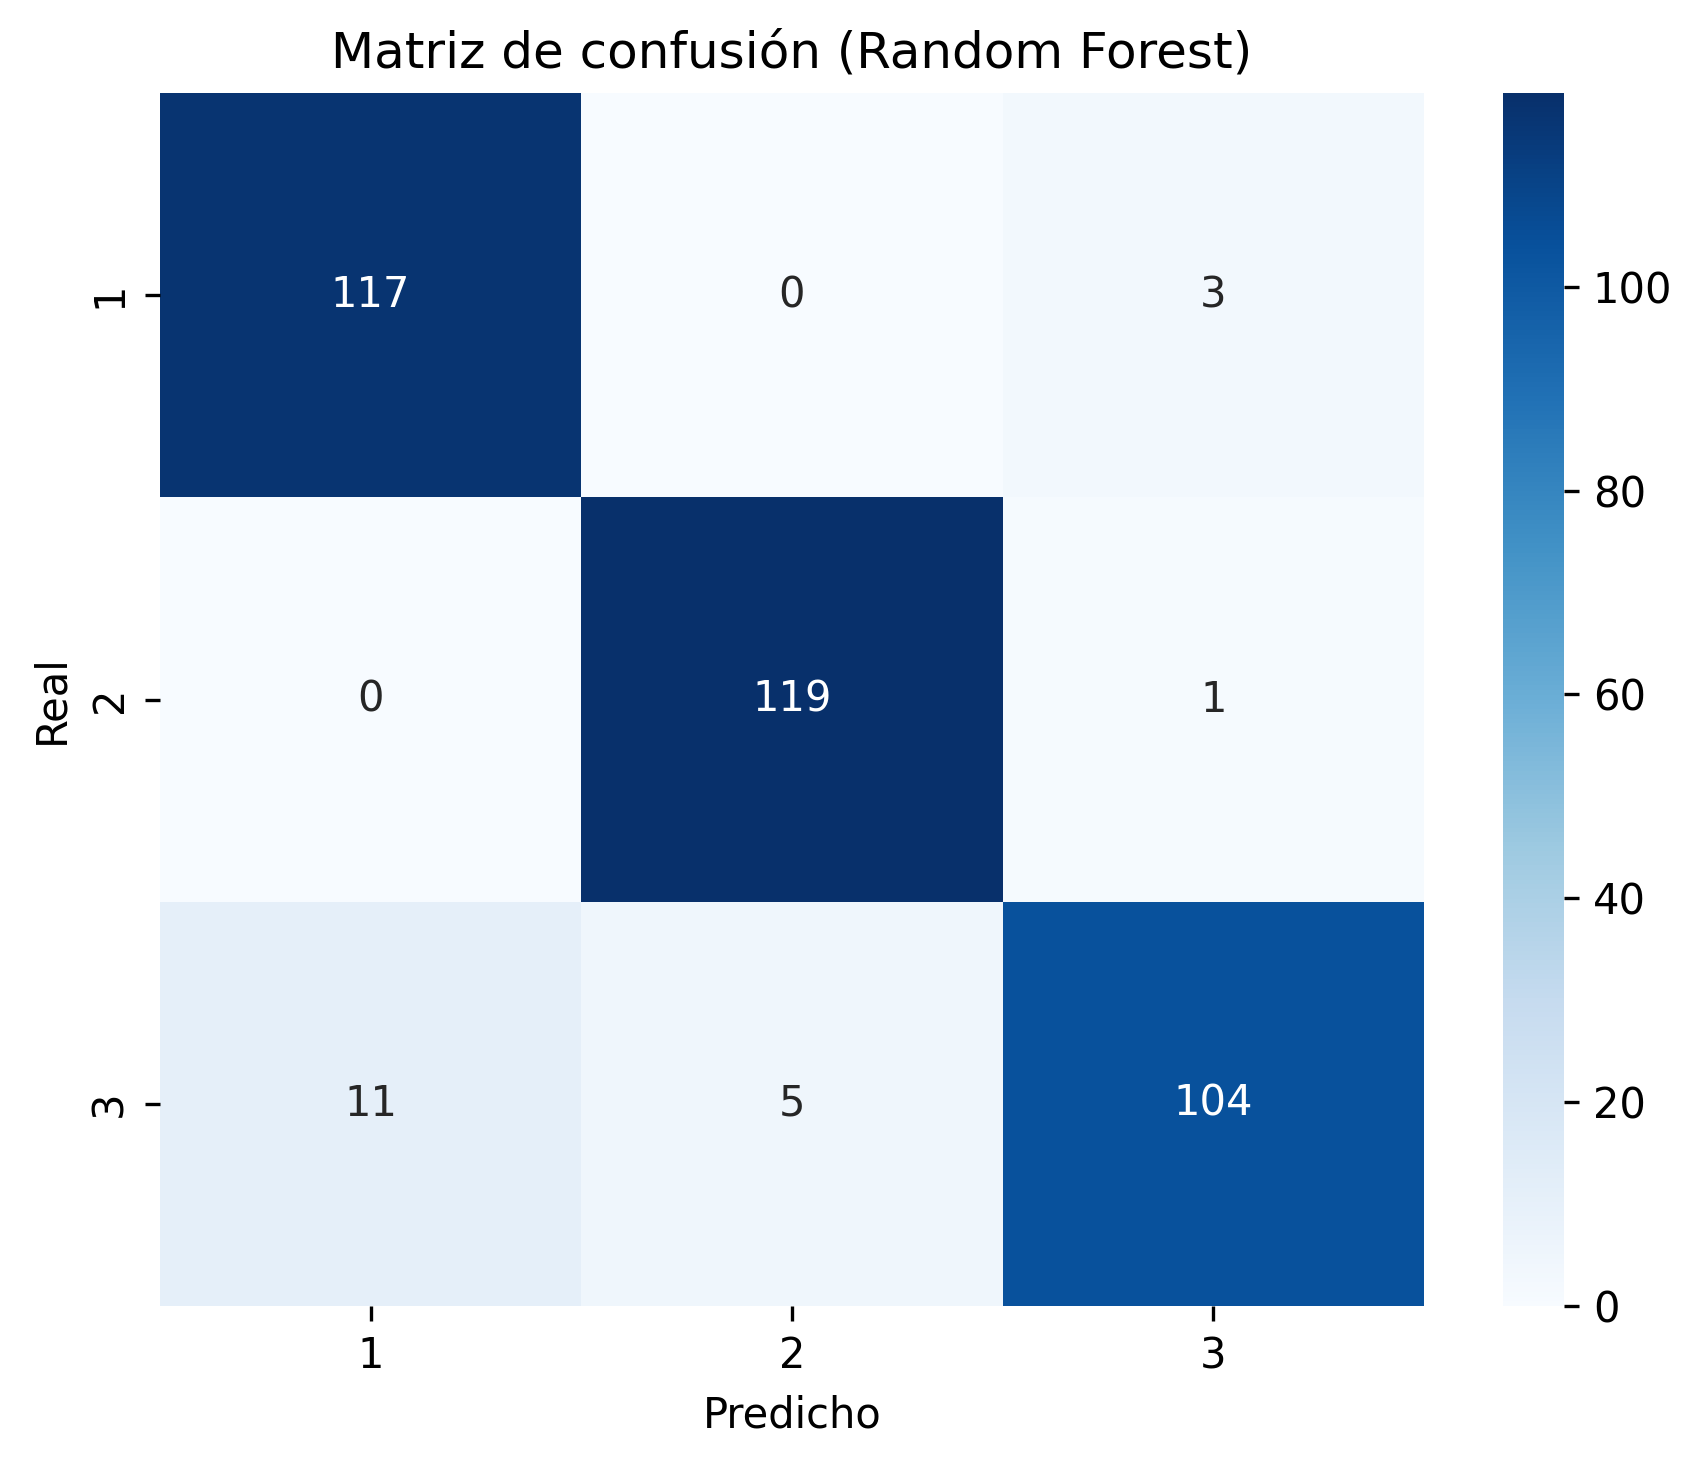
\includegraphics[width=0.7\linewidth]{confusion_matrix_rf.png}
    \caption{Confusion Matrix for random forest with bilateral features.}
    \label{fig:cm_rf}
\end{figure}

The feature importance plot for Random Forest with bilateral features indicates the relative contribution of each kinematic variable to the classification performance.

\begin{figure}[h]
    \centering
    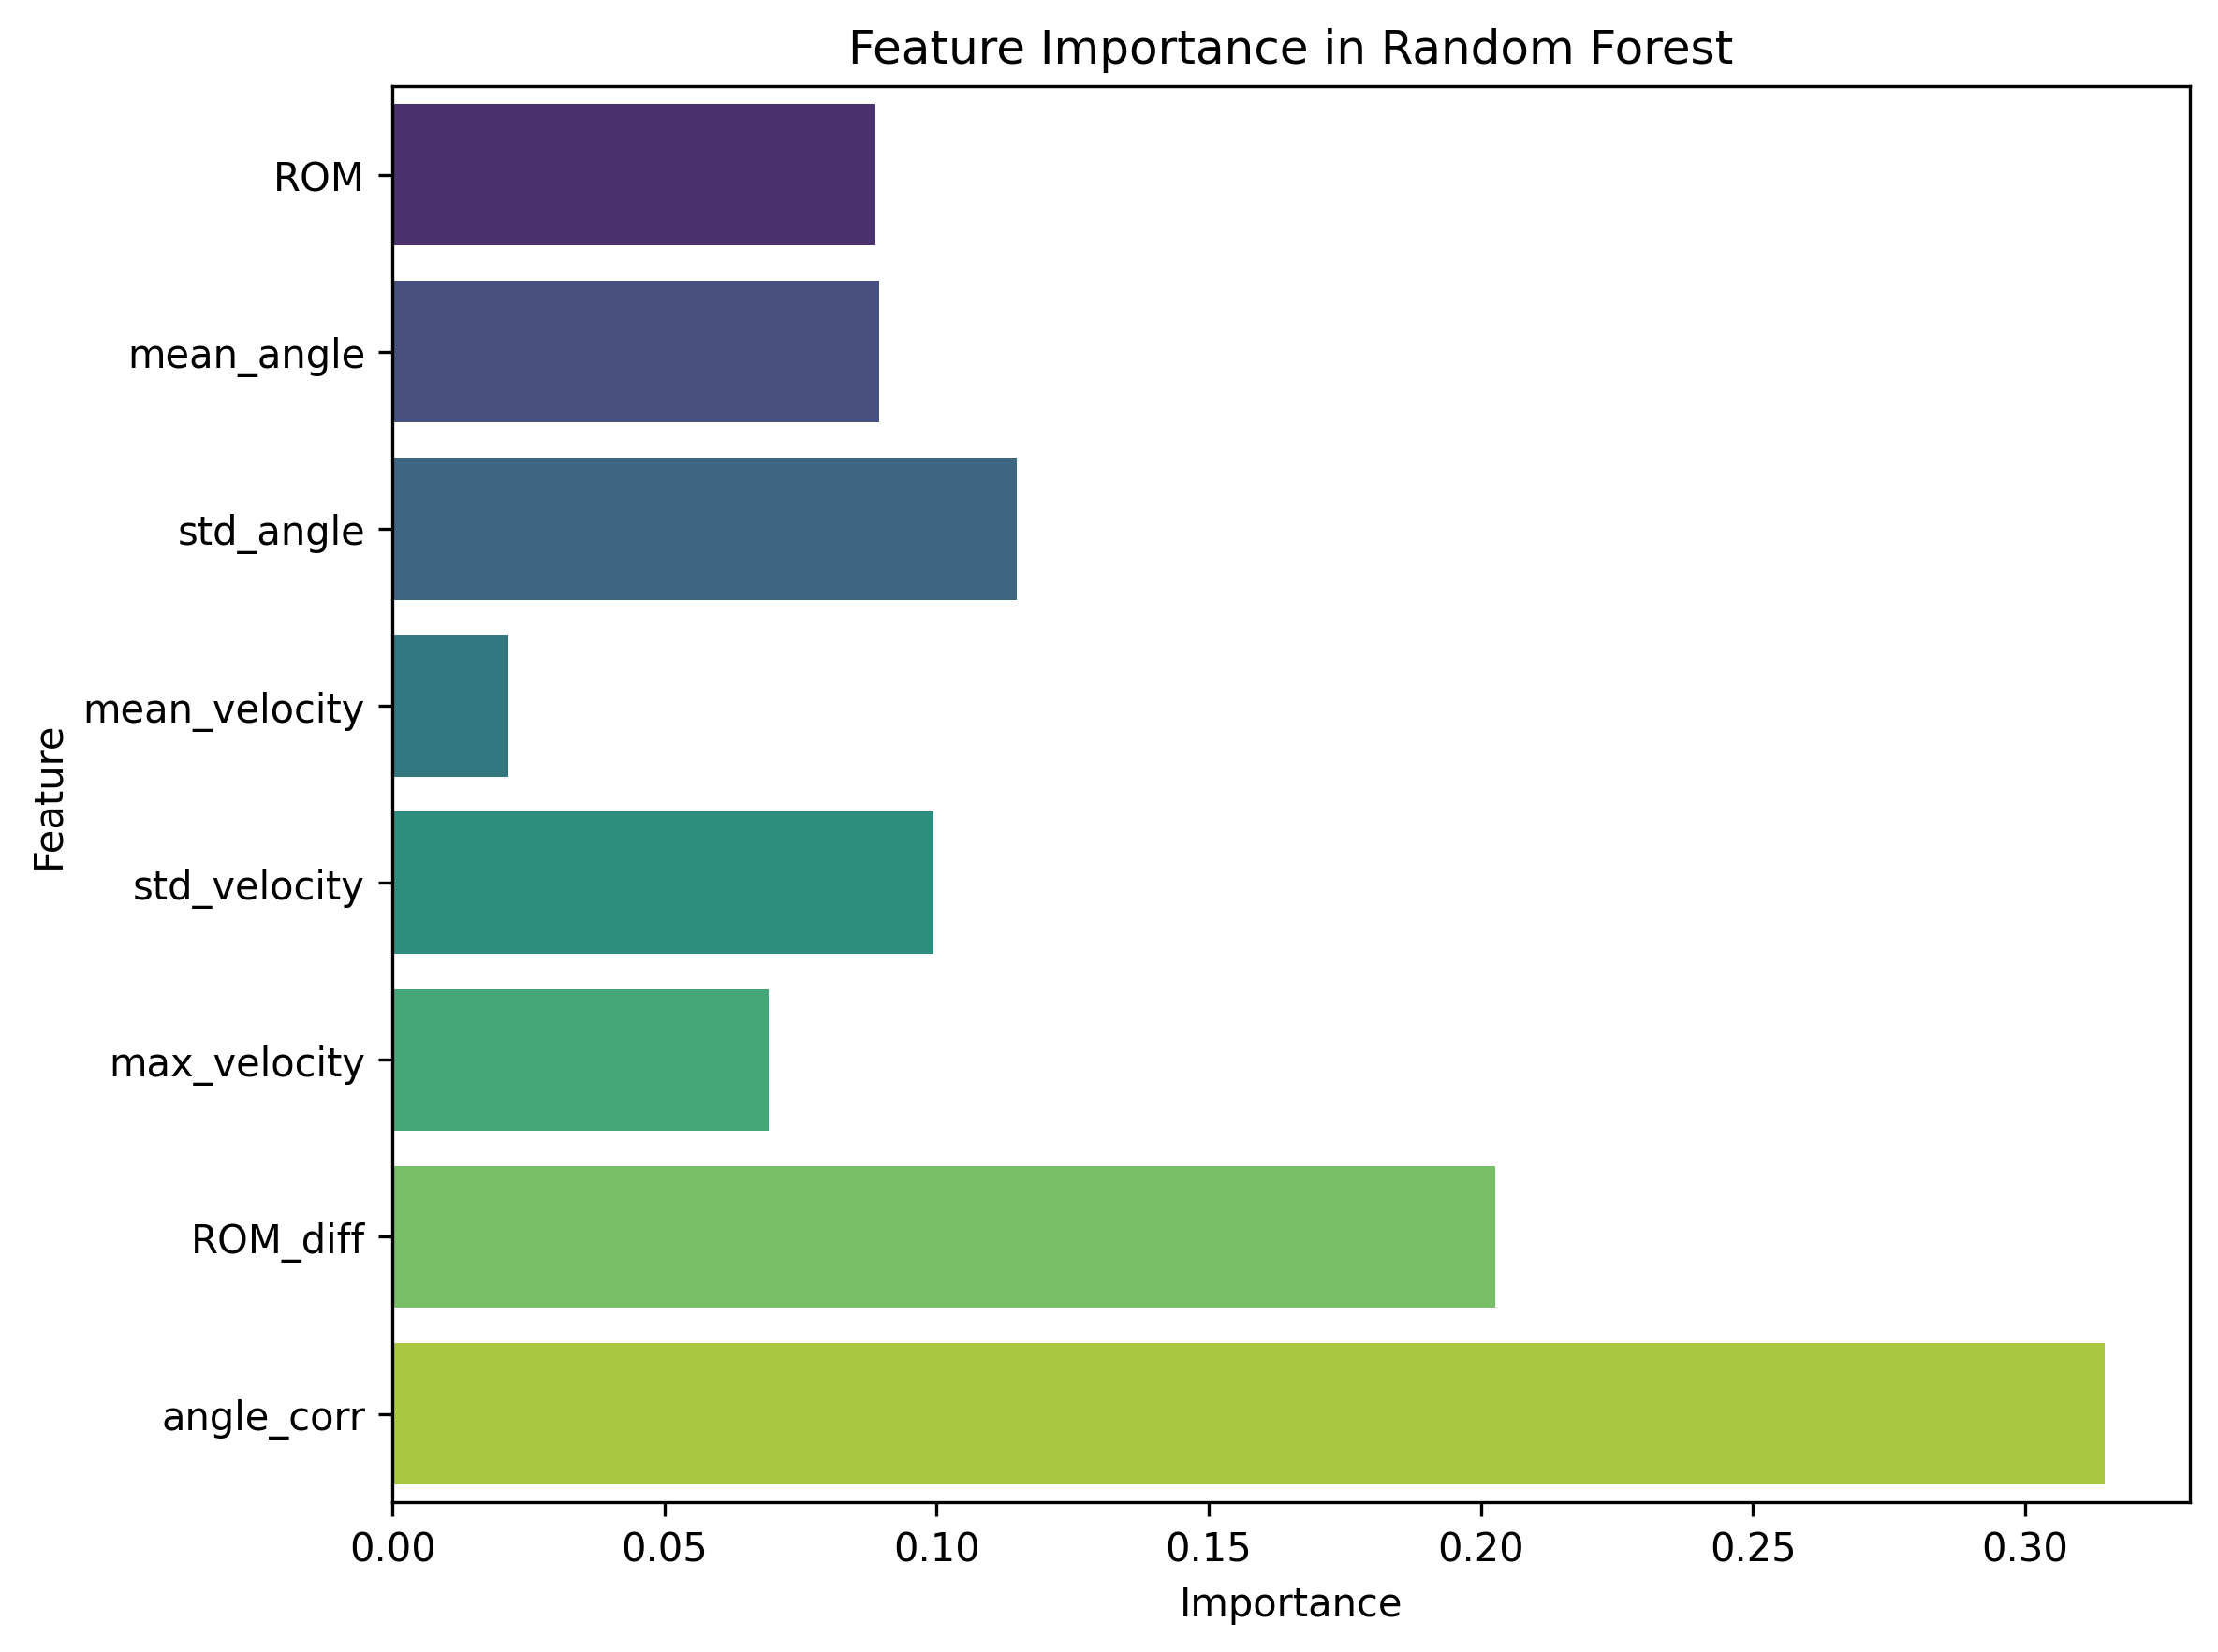
\includegraphics[width=0.7\linewidth]{importance_features_rf.png}
    \caption{Features importance for random forest with bilateral features.}
    \label{fig:importance_rf}
\end{figure}

The confusion matrix for the Support Vector Machine (SVM) trained with bilateral features demonstrates the separability achieved by the kernel-based approach.

\begin{figure}[h]
    \centering
    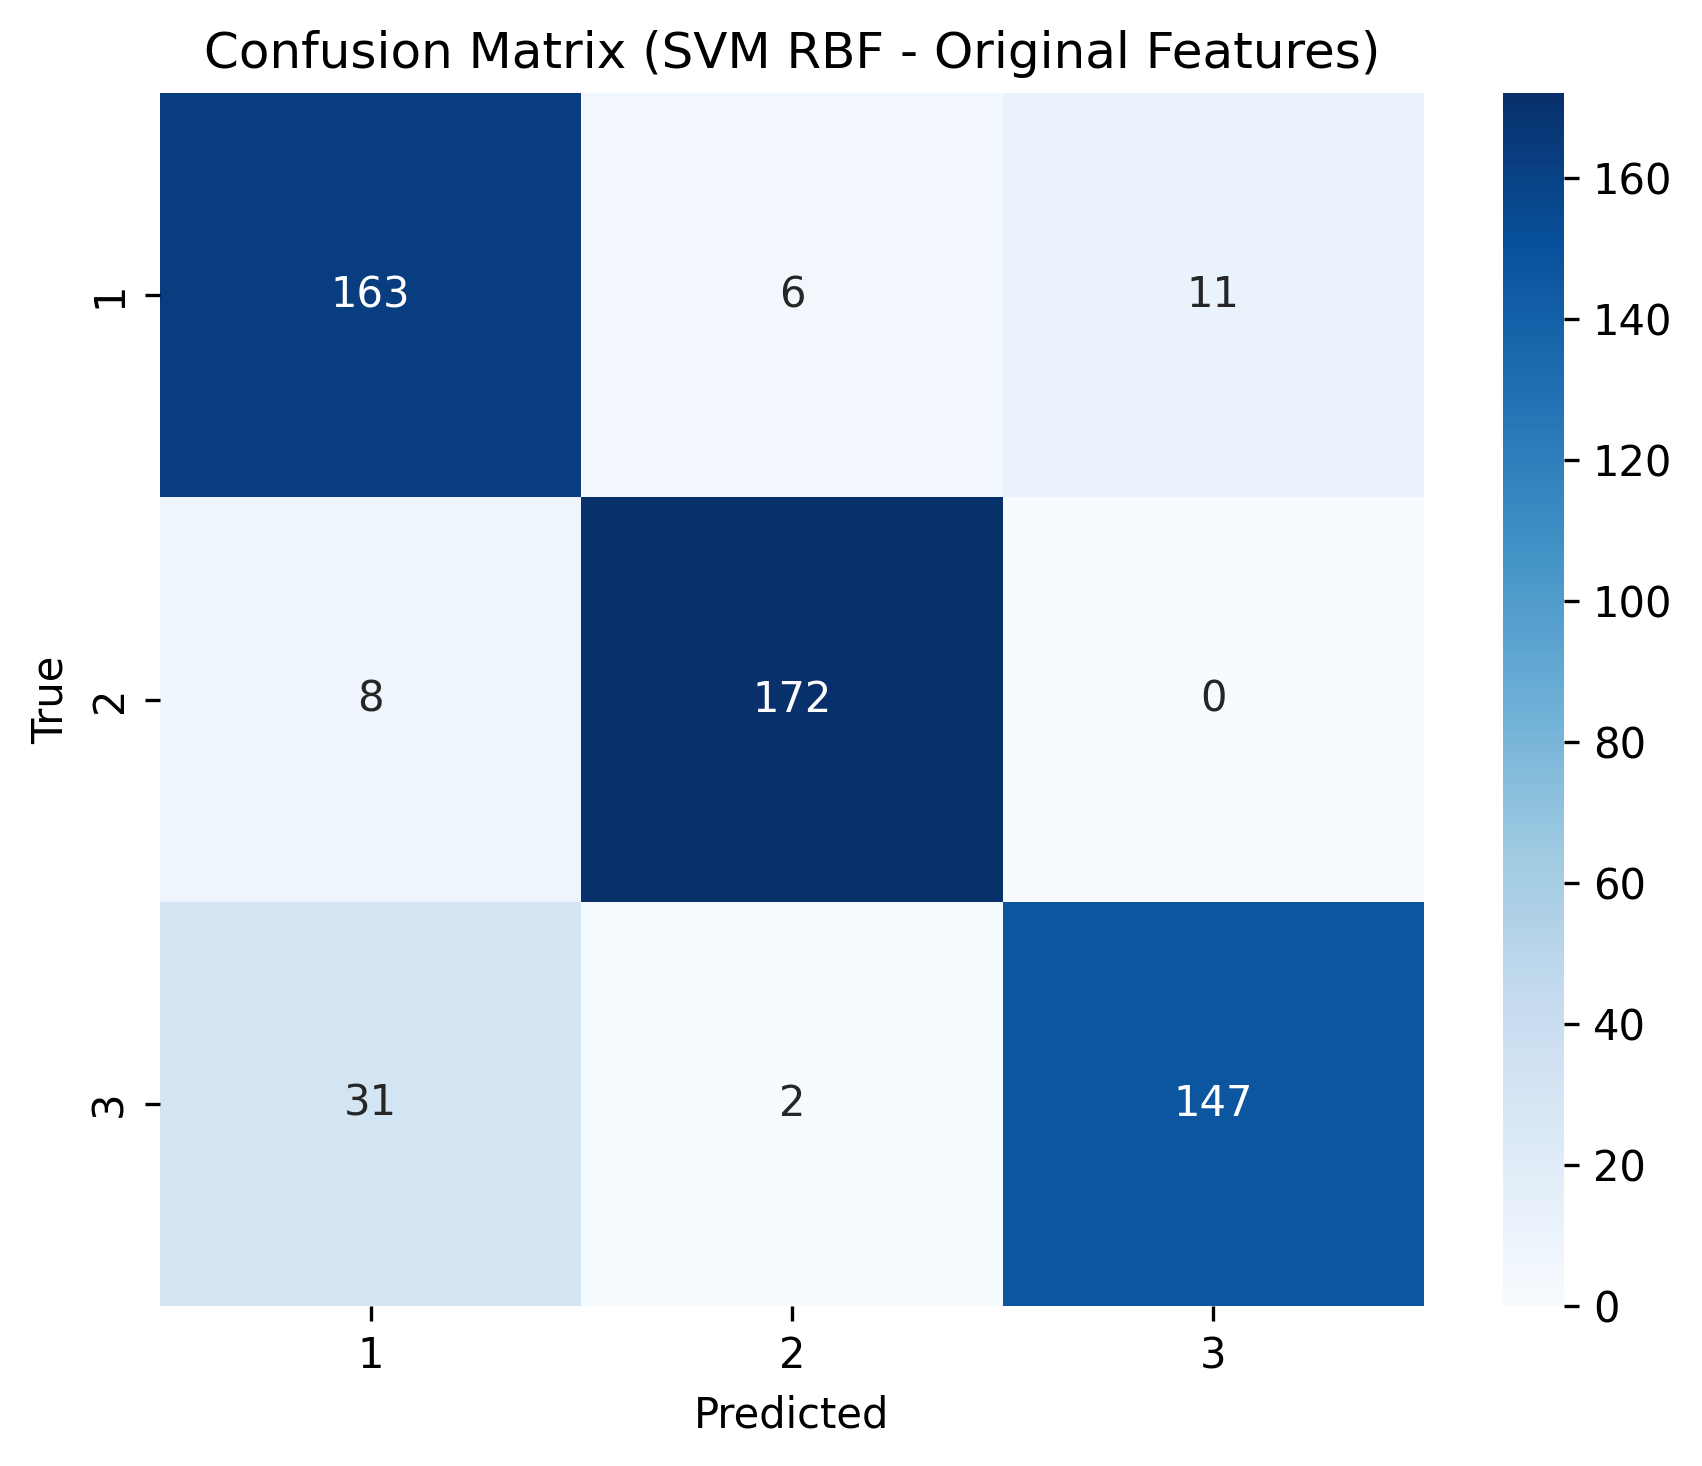
\includegraphics[width=0.7\linewidth]{confusion_matrix_svm.png}
    \caption{Confusion Matrix for SVM with bilateral features.}
    \label{fig:cm_svm}
\end{figure}

The confusion matrix for the Multi-Layer Perceptron (MLP) using angle and velocity statistics shows the performance of the neural network in capturing nonlinear relationships among gait features.

\begin{figure}[h]
    \centering
    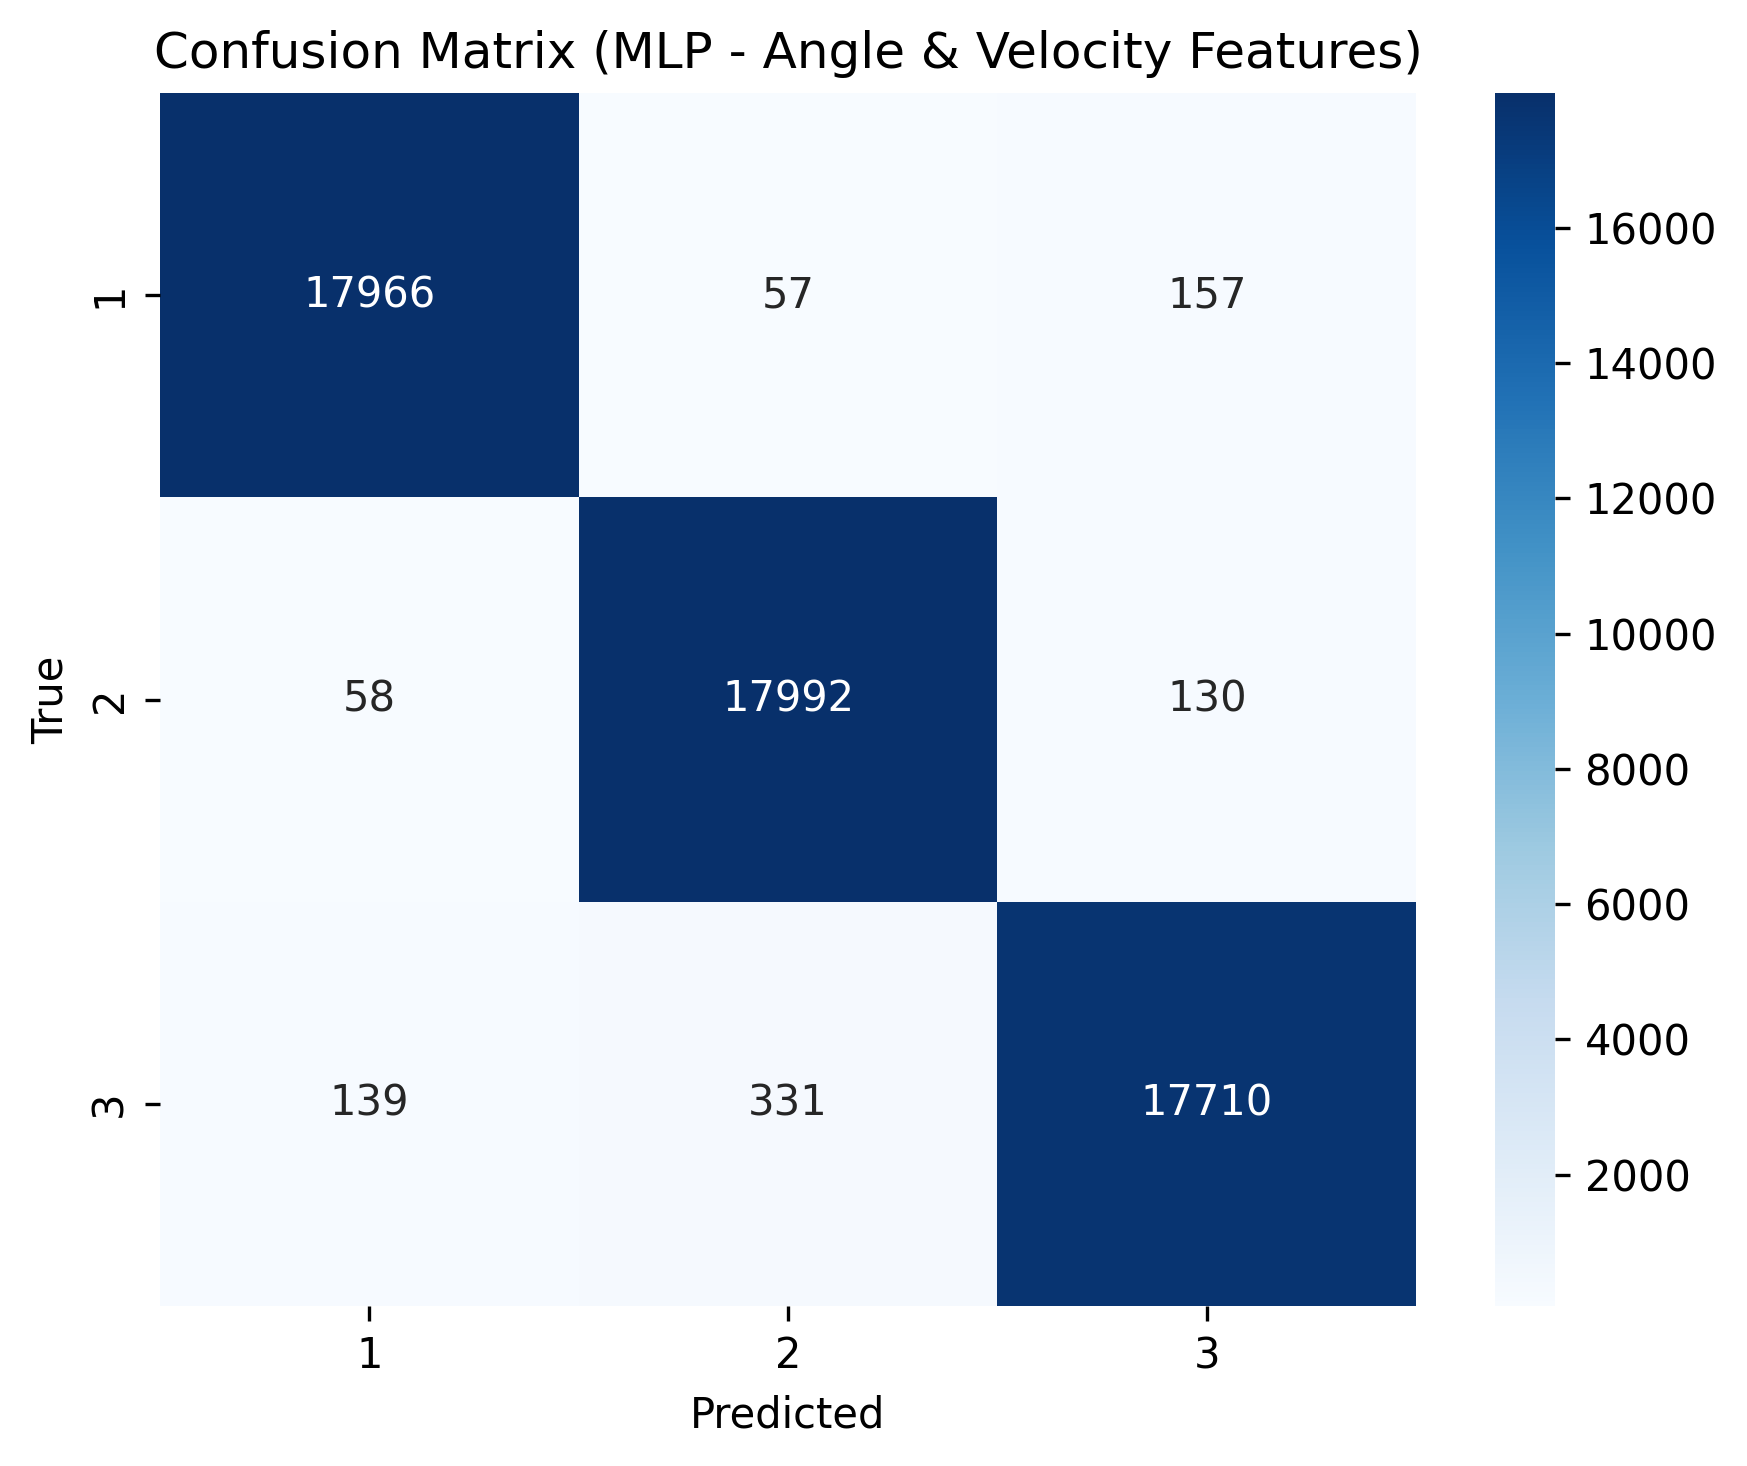
\includegraphics[width=0.7\linewidth]{confusion_matrix_MLP.png}
    \caption{Confusion Matrix for MLP using angle and velocity basic statistics.}
    \label{fig:cm_mlp}
\end{figure}


\subsection{Visualization of Feature Separability}

To further validate the discriminative power of bilateral features, PCA projections were generated. Figure~\ref{fig:pca} shows the 3D scatterplot of principal components,
colored by condition. The inclusion of \texttt{ROM\_diff} and \texttt{angle\_corr} produced clear separability between classes, confirming their importance in classification, 
even when the classes seem to be mixed on the 3D PCA, or in the ROM vs Condition plots as is swhon in fig \ref{fig:romvscondition}. It can be confirmed in the boxplot presented 
in the figure \ref{fig:importance_rf} and figure \ref{fig:anglecorrvscondition}, in comparioson with the general ROM (ROM of left leg and right leg) vs condition, where no significant 
differences can be perceived. 

\begin{figure}[h]
    \centering
    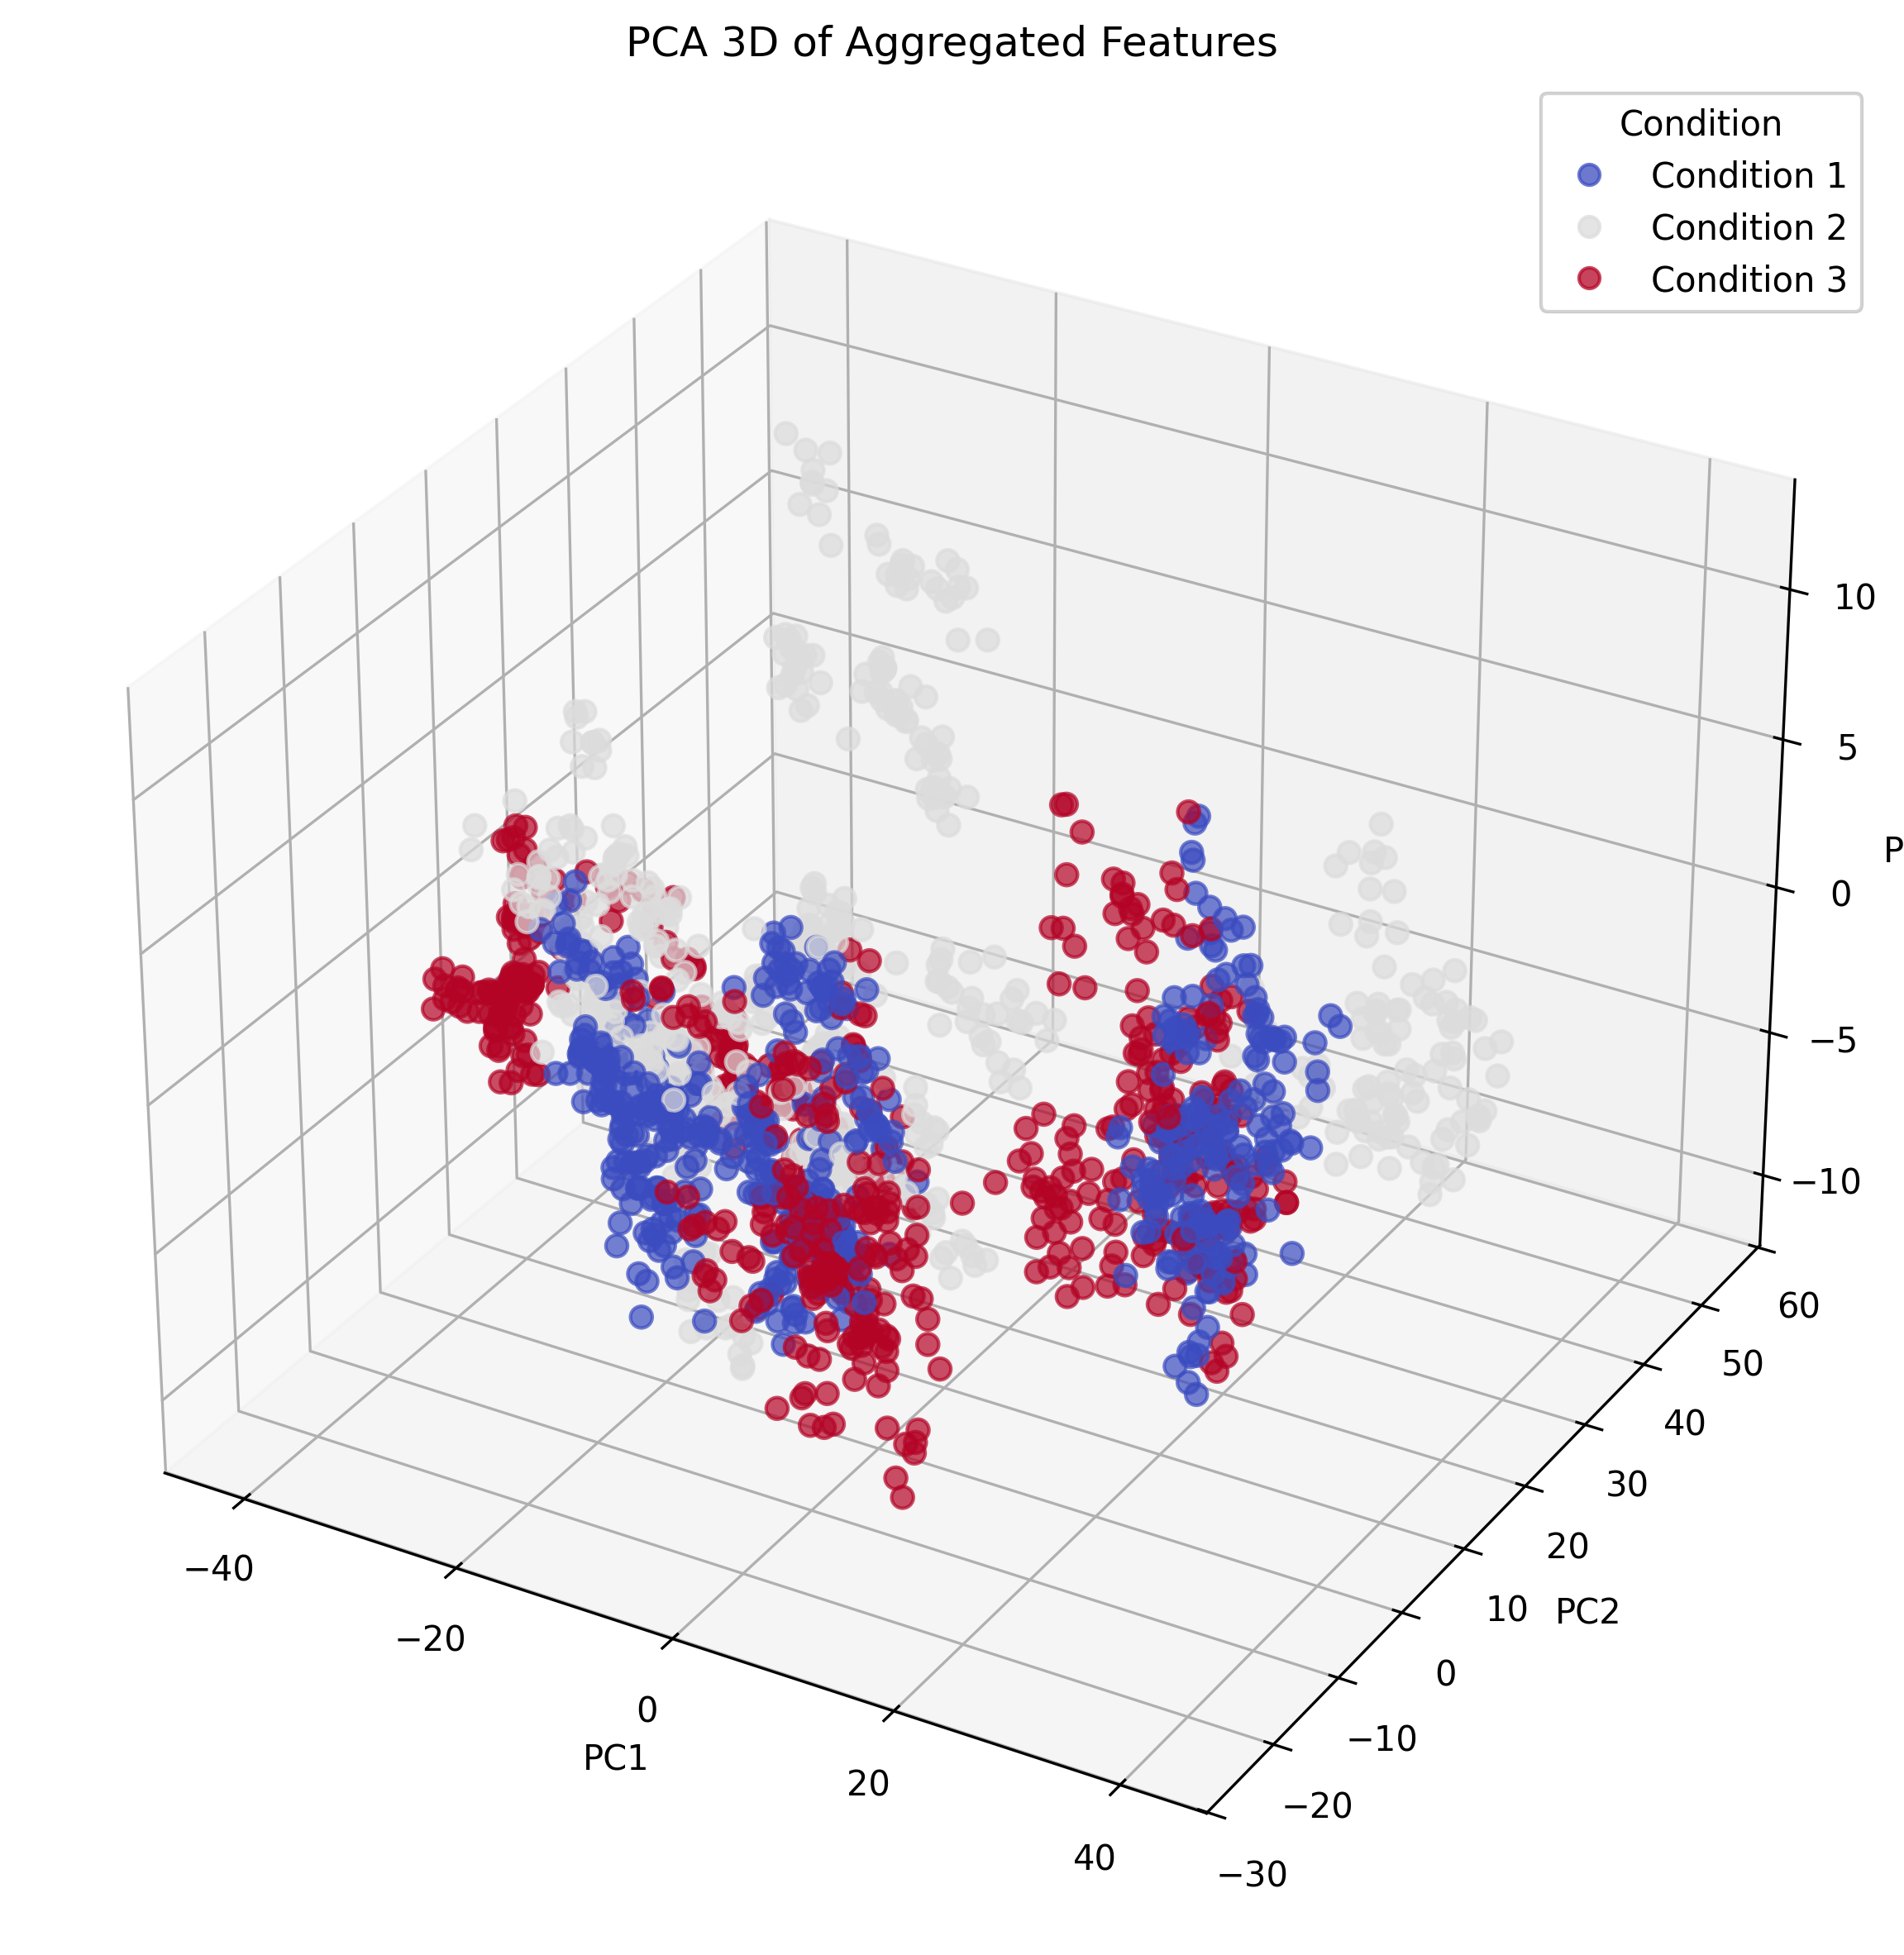
\includegraphics[width=0.8\linewidth]{svm_pca_2D.png}
    \caption{PCA 3D projection of bilateral features showing separability across conditions.}
    \label{fig:pca}
\end{figure}

\begin{figure}
    \centering
    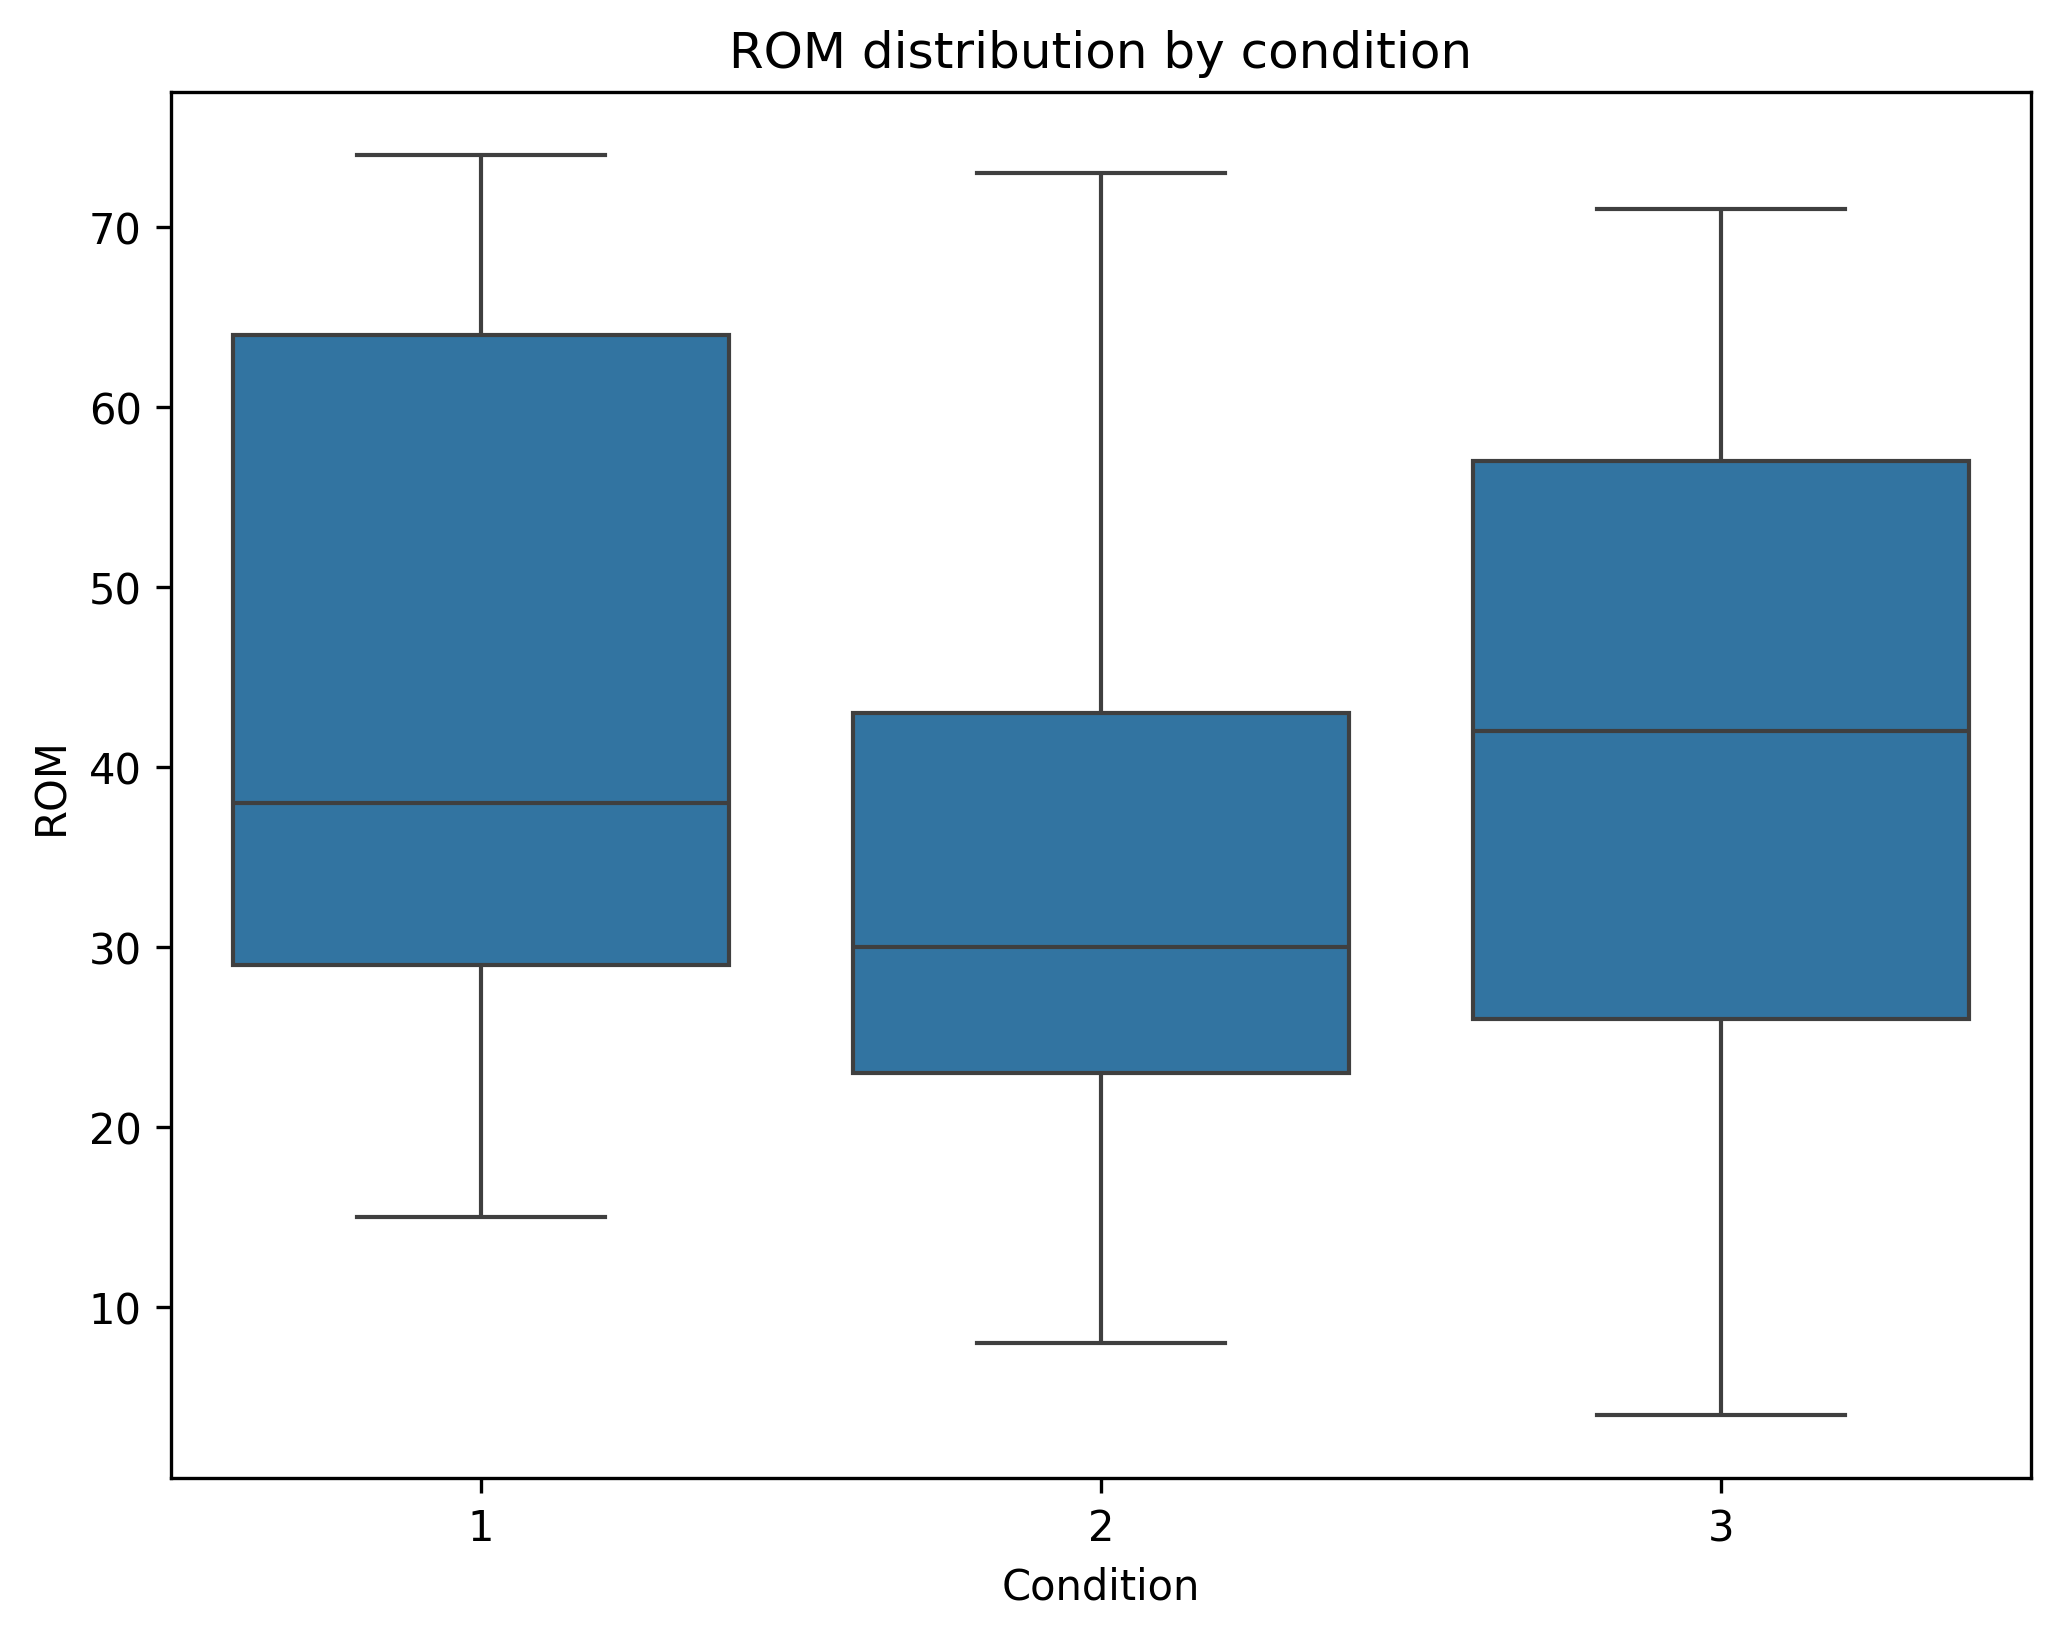
\includegraphics[width=0.8\linewidth]{ROM_condition.png}
    \caption{Bilateral ROM vs condition.}
    \label{fig:romvscondition}
\end{figure}

\begin{figure}
    \centering
    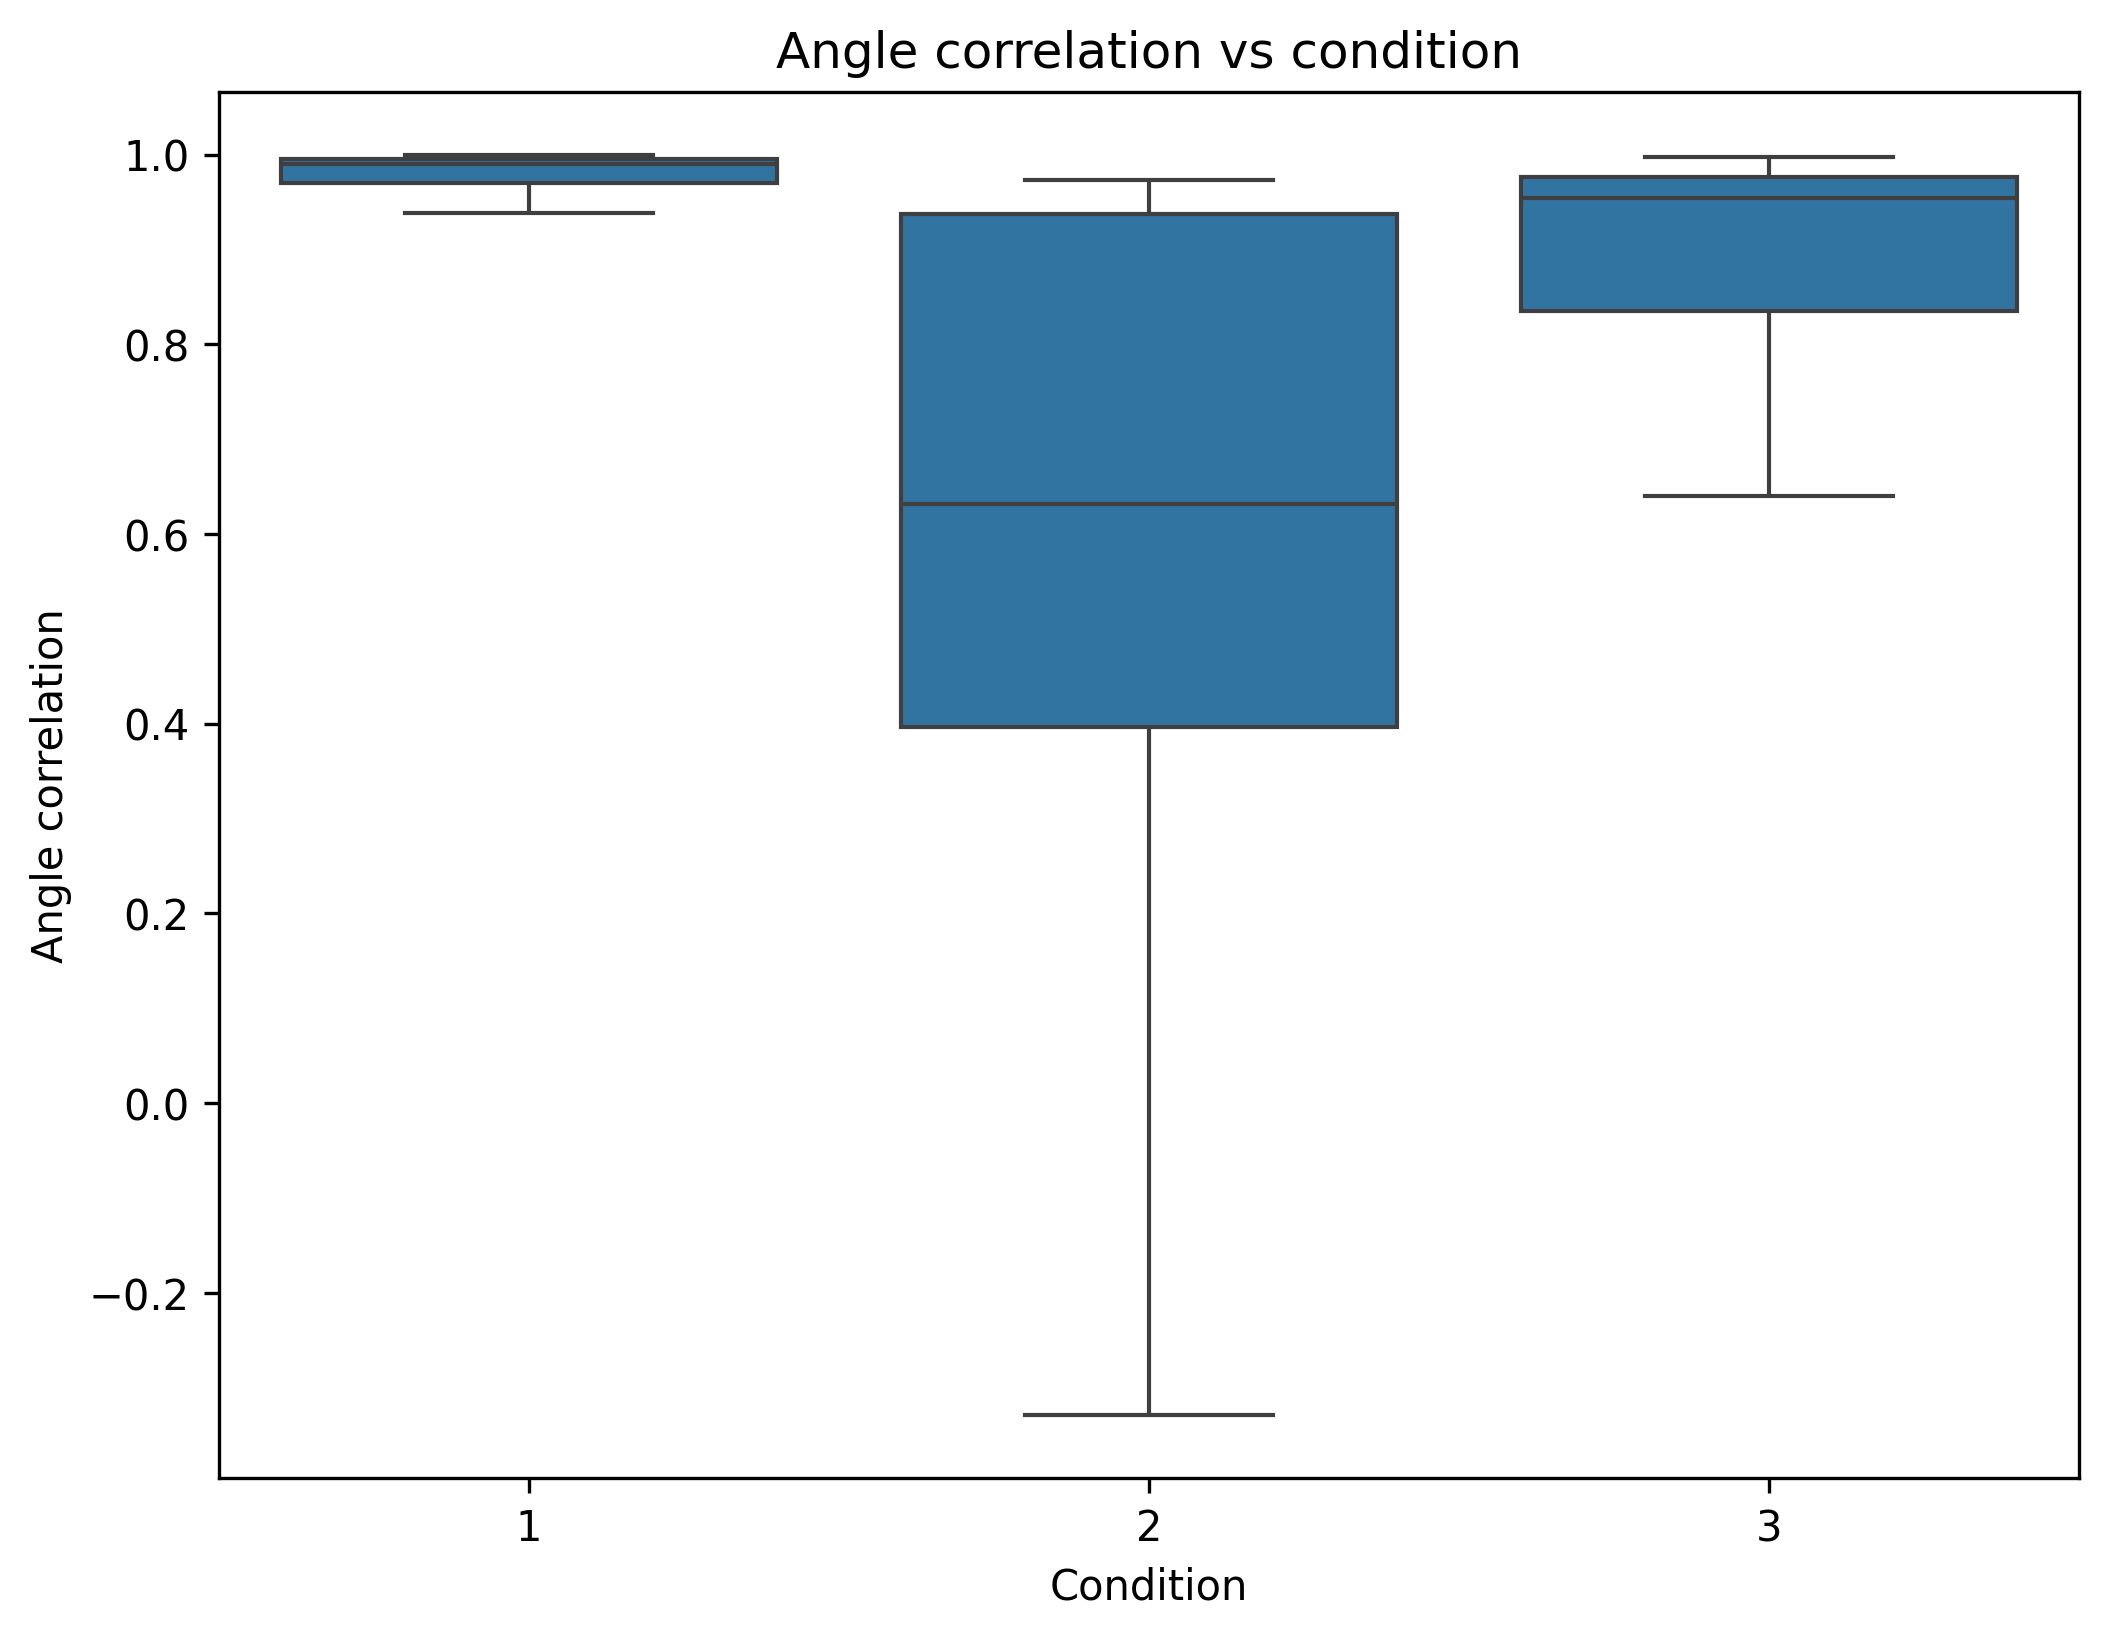
\includegraphics[width=0.8\linewidth]{anglecorr_condition.png}
    \caption{Angle correlation vs condition.}
    \label{fig:anglecorrvscondition}
\end{figure}


\subsection{Summary}
The results demonstrate that:
\begin{itemize}
    \item Classical models (Logistic Regression, KNN, Random Forest) achieved solid baselines.
    \item SVM benefited significantly from bilateral features, achieving high accuracy and balanced class performance.
    \item Neural networks (MLP) achieved near-perfect accuracy, confirming the hypothesis that angle and velocity features contain sufficient discriminative information.
    \item Confusion matrices illustrate minimal misclassification, with most errors concentrated in condition 3.
\end{itemize}

\section{Discussion}

The comparative evaluation of machine learning models highlights the decisive role of bilateral asymmetry features in gait classification. While traditional metrics such as ROM, 
mean angle, and velocity provided a solid baseline, they were insufficient to fully capture the discriminative patterns between conditions. The introduction of engineered 
features (\texttt{ROM\_diff}, \texttt{angle\_corr}) substantially improved performance across classifiers, confirming the hypothesis  that inter-limb differences are critical 
markers of gait abnormalities.

Support Vector Machines (SVM) demonstrated strong performance, particularly when trained per joint, with the knee and ankle joints contributing most to separability. 
This aligns with clinical observations that these joints are more sensitive to bracing and pathological conditions. Random Forests provided interpretability through feature 
importance rankings, which consistently placed bilateral descriptors at the top, reinforcing their relevance. KNN achieved moderate accuracy, reflecting its reliance on local 
neighborhood structures, which may be less effective in high-dimensional feature spaces.

Logistic Regression, while mathematically elegant and interpretable, struggled to capture the non-linear separability inherent in the dataset. In contrast, the Multi-Layer 
Perceptron (MLP) achieved near-perfect accuracy, demonstrating the capacity of neural networks to model complex biomechanical relationships even when engineered are no provided
features. The confusion matrices confirmed minimal misclassification, with most errors concentrated in condition 3, suggesting that this class exhibits more subtle variability.

The unsupervised KMeans clustering provided complementary validation, showing that conditions naturally separate when only angle correlation feature is included. This indicates that 
asymmetry descriptors not only improve supervised classification but also reveal intrinsic structure in the data as is showing in the figure \ref{fig:anglecorrvscondition}.

As is shown in the table \ref{tab:joint_results} it demonstrates that supervised learning algorithms consistently
outperform unsupervised clustering. Logistic Regression and SVM achieved high accuracy and balanced macro-F1 scores for every joint, with Joint~1 reaching values above 0.96.
These results confirm that supervised approaches are better suited for capturing the discriminative patterns present in the biomechanical data, regardless 
of the joint analyzed. Overall, the supervised models provide more reliable and interpretable performance across all joints compared to the unsupervised baseline.

\section{Conclusion}

This study presents a modular machine learning pipeline for gait analysis, integrating classical algorithms and neural networks with domain-inspired feature engineering. 
The results demonstrate that bilateral asymmetry features are decisive in improving classification accuracy, elevating performance from strong baselines to near-perfect results with MLPs.
These findings highlight the importance of incorporating biomechanical insights into feature design, rather than relying solely on raw kinematic data.

The contributions of this work are threefold: (i) the design of a reproducible pipeline for gait feature extraction and classification, (ii) the comparative analysis of 
multiple machine learning models with their mathematical foundations, and (iii) the demonstration that bilateral asymmetry features substantially enhance performance. 

Future work will extend this pipeline to larger datasets and explore real-time applications in rehabilitation robotics. Additionally, GPU-accelerated neural networks may
allow for deeper architectures and faster training, further enhancing the potential of machine learning in biomechanical diagnostics. The integration of asymmetry-aware models into 
clinical practice could provide more accurate assessments of patient mobility and support the development of personalized rehabilitation strategies.

\begin{thebibliography}{99}

\bibitem{winter1991biomechanics}
D.~A. Winter,
\emph{Biomechanics and Motor Control of Human Movement}.
Wiley, 1991.

\bibitem{whittle2007gait}
M.~Whittle, \emph{Gait Analysis: An Introduction}. Butterworth-Heinemann, 2007.

\bibitem{bishop2006pattern}
C.~M. Bishop,
\emph{Pattern Recognition and Machine Learning}.
Springer, 2006.

\bibitem{murphy2012machine}
K.~P. Murphy,
\emph{Machine Learning: A Probabilistic Perspective}.
MIT Press, 2012.

\bibitem{gait_asymmetry}
H.~Sadeghi, F.~Prince, S.~Sadeghi, and H.~Labelle,
``Symmetry and asymmetry in human gait: a review,''
\emph{Gait \& Posture}, vol.~12, no.~1, pp.~34--45, 2000.

\bibitem{helwig2022gait}
N.~Helwig and E.~Hsiao-Wecksler,
``Multivariate Gait Data,''
\emph{UCI Machine Learning Repository},
2022. Available: \url{https://doi.org/10.24432/C5861T}

\bibitem{rampp2015}
A.~Rampp, S.~Barth, C.~Schneider, et al., 
``Inertial sensor-based stride parameter calculation from gait sequences in geriatric patients,'' 
\emph{IEEE Transactions on Biomedical Engineering}, vol.~62, no.~4, pp.~1089--1097, 2015.

\bibitem{cox1958}
D.~R. Cox,
``The regression analysis of binary sequences,''
\emph{Journal of the Royal Statistical Society: Series B (Methodological)}, 
vol.~20, no.~2, pp.~215--242, 1958.

\bibitem{cover1967}
T.~M. Cover and P.~E. Hart,
``Nearest neighbor pattern classification,''
\emph{IEEE Transactions on Information Theory}, vol.~13, no.~1, pp.~21--27, 1967.

\bibitem{breiman2001}
L.~Breiman, 
``Random forests,'' 
\emph{Machine Learning}, vol.~45, no.~1, pp.~5--32, 2001.

\bibitem{cortes1995}
C.~Cortes and V.~Vapnik, 
``Support-vector networks,'' 
\emph{Machine Learning}, vol.~20, no.~3, pp.~273--297, 1995.

\bibitem{jain2010}
A.~K. Jain, 
``Data clustering: 50 years beyond K-means,'' 
\emph{Pattern Recognition Letters}, vol.~31, no.~8, pp.~651--666, 2010.

\bibitem{rumelhart1986}
D.~E. Rumelhart, G.~E. Hinton, and R.~J. Williams, 
``Learning representations by back-propagating errors,'' 
\emph{Nature}, vol.~323, pp.~533--536, 1986.

\end{thebibliography}
\end{document}

